\documentclass[a4paper]{article}

%=========================================
% Packages
%=========================================
\usepackage{mathtools}
\usepackage{amsfonts}
\usepackage{amsmath}
\usepackage{amssymb}
\usepackage{amsthm}
\usepackage[a4paper, total={6in, 8in}, margin=1in]{geometry}
\usepackage[utf8]{inputenc}
\usepackage{fancyhdr}
\usepackage[utf8]{inputenc}
\usepackage{graphicx}
\usepackage{physics}
\usepackage[listings]{tcolorbox}
\usepackage{hyperref}
\usepackage{tikz-cd}
\usepackage{adjustbox}
\usepackage{enumitem}
\usepackage[font=small,labelfont=bf]{caption}
\usepackage{subcaption}
\usepackage{wrapfig}
\usepackage{makecell}



\raggedright

\usetikzlibrary{arrows.meta}

\DeclarePairedDelimiter\ceil{\lceil}{\rceil}
\DeclarePairedDelimiter\floor{\lfloor}{\rfloor}

%=========================================
% Fonts
%=========================================
\usepackage{tgpagella}
\usepackage[T1]{fontenc}


%=========================================
% Custom Math Operators
%=========================================
\DeclareMathOperator{\adj}{adj}
\DeclareMathOperator{\im}{im}
\DeclareMathOperator{\nullity}{nullity}
\DeclareMathOperator{\sign}{sign}
\DeclareMathOperator{\dom}{dom}
\DeclareMathOperator{\lcm}{lcm}
\DeclareMathOperator{\ran}{ran}
\DeclareMathOperator{\ext}{Ext}
\DeclareMathOperator{\dist}{dist}
\DeclareMathOperator{\diam}{diam}
\DeclareMathOperator{\aut}{Aut}
\DeclareMathOperator{\inn}{Inn}
\DeclareMathOperator{\syl}{Syl}
\DeclareMathOperator{\edo}{End}
\DeclareMathOperator{\cov}{Cov}
\DeclareMathOperator{\vari}{Var}
\DeclareMathOperator{\cha}{char}
\DeclareMathOperator{\Span}{span}
\DeclareMathOperator{\ord}{ord}
\DeclareMathOperator{\res}{res}
\DeclareMathOperator{\Hom}{Hom}
\DeclareMathOperator{\Mor}{Mor}
\DeclareMathOperator{\coker}{coker}
\DeclareMathOperator{\Obj}{Obj}
\DeclareMathOperator{\id}{id}
\DeclareMathOperator{\GL}{GL}
\DeclareMathOperator*{\colim}{colim}

%=========================================
% Custom Commands (Shortcuts)
%=========================================
\newcommand{\CP}{\mathbb{CP}}
\newcommand{\GG}{\mathbb{G}}
\newcommand{\F}{\mathbb{F}}
\newcommand{\N}{\mathbb{N}}
\newcommand{\Q}{\mathbb{Q}}
\newcommand{\R}{\mathbb{R}}
\newcommand{\C}{\mathbb{C}}
\newcommand{\E}{\mathbb{E}}
\newcommand{\Prj}{\mathbb{P}}
\newcommand{\RP}{\mathbb{RP}}
\newcommand{\T}{\mathbb{T}}
\newcommand{\Z}{\mathbb{Z}}
\newcommand{\A}{\mathbb{A}}
\renewcommand{\H}{\mathbb{H}}
\newcommand{\K}{\mathbb{K}}

\newcommand{\mA}{\mathcal{A}}
\newcommand{\mB}{\mathcal{B}}
\newcommand{\mC}{\mathcal{C}}
\newcommand{\mD}{\mathcal{D}}
\newcommand{\mE}{\mathcal{E}}
\newcommand{\mF}{\mathcal{F}}
\newcommand{\mG}{\mathcal{G}}
\newcommand{\mH}{\mathcal{H}}
\newcommand{\mI}{\mathcal{I}}
\newcommand{\mJ}{\mathcal{J}}
\newcommand{\mK}{\mathcal{K}}
\newcommand{\mL}{\mathcal{L}}
\newcommand{\mM}{\mathcal{M}}
\newcommand{\mO}{\mathcal{O}}
\newcommand{\mP}{\mathcal{P}}
\newcommand{\mS}{\mathcal{S}}
\newcommand{\mT}{\mathcal{T}}
\newcommand{\mV}{\mathcal{V}}
\newcommand{\mW}{\mathcal{W}}

%=========================================
% Colours!!!
%=========================================
\definecolor{LightBlue}{HTML}{2D64A6}
\definecolor{ForestGreen}{HTML}{4BA150}
\definecolor{DarkBlue}{HTML}{000080}
\definecolor{LightPurple}{HTML}{cc99ff}
\definecolor{LightOrange}{HTML}{ffc34d}
\definecolor{Buff}{HTML}{DDAE7E}
\definecolor{Sunset}{HTML}{F2C57C}
\definecolor{Wenge}{HTML}{584B53}
\definecolor{Coolgray}{HTML}{9098CB}
\definecolor{Lavender}{HTML}{D6E3F8}
\definecolor{Glaucous}{HTML}{828BC4}
\definecolor{Mauve}{HTML}{C7A8F0}
\definecolor{Darkred}{HTML}{880808}
\definecolor{Beaver}{HTML}{9A8873}
\definecolor{UltraViolet}{HTML}{52489C}



%=========================================
% Theorem Environment
%=========================================
\tcbuselibrary{listings, theorems, breakable, skins}

\newtcbtheorem[number within = subsection]{thm}{Theorem}%
{	colback=Buff!3, 
	colframe=Buff, 
	fonttitle=\bfseries, 
	breakable, 
	enhanced jigsaw, 
	halign=left
}{thm}

\newtcbtheorem[number within=subsection, use counter from=thm]{defn}{Definition}%
{  colback=cyan!1,
    colframe=cyan!50!black,
	fonttitle=\bfseries, breakable, 
	enhanced jigsaw, 
	halign=left
}{defn}

\newtcbtheorem[number within=subsection, use counter from=thm]{axm}{Axiom}%
{	colback=red!5, 
	colframe=Darkred, 
	fonttitle=\bfseries, 
	breakable, 
	enhanced jigsaw, 
	halign=left
}{axm}

\newtcbtheorem[number within=subsection, use counter from=thm]{prp}{Proposition}%
{	colback=LightBlue!3, 
	colframe=Glaucous, 
	fonttitle=\bfseries, 
	breakable, 
	enhanced jigsaw, 
	halign=left
}{prp}

\newtcbtheorem[number within=subsection, use counter from=thm]{lmm}{Lemma}%
{	colback=LightBlue!3, 
	colframe=LightBlue!60, 
	fonttitle=\bfseries, 
	breakable, 
	enhanced jigsaw, 
	halign=left
}{lmm}

\newtcbtheorem[number within=subsection, use counter from=thm]{crl}{Corollary}%
{	colback=LightBlue!3, 
	colframe=LightBlue!60, 
	fonttitle=\bfseries, 
	breakable, 
	enhanced jigsaw, 
	halign=left
}{crl}

\newtcbtheorem[number within=subsection, use counter from=thm]{eg}{Example}%
{	colback=Beaver!5, 
	colframe=Beaver, 
	fonttitle=\bfseries, 
	breakable, 
	enhanced jigsaw, 
	halign=left
}{eg}

\newtcbtheorem[number within=subsection, use counter from=thm]{ex}{Exercise}%
{	colback=Beaver!5, 
	colframe=Beaver, 
	fonttitle=\bfseries, 
	breakable, 
	enhanced jigsaw, 
	halign=left
}{ex}

\newtcbtheorem[number within=subsection, use counter from=thm]{alg}{Algorithm}%
{	colback=UltraViolet!5, 
	colframe=UltraViolet, 
	fonttitle=\bfseries, 
	breakable, 
	enhanced jigsaw, 
	halign=left
}{alg}




%=========================================
% Hyperlinks
%=========================================
\hypersetup{
    colorlinks=true, %set true if you want colored links
    linktoc=all,     %set to all if you want both sections and subsections linked
    linkcolor=DarkBlue,  %choose some color if you want links to stand out
}


\pagestyle{fancy}
\fancyhf{}
\rhead{Labix}
\lhead{Algebraic Topology 1}
\rfoot{\thepage}

\title{Algebraic Topology 1}

\author{Labix}

\date{\today}
\begin{document}
\maketitle
\begin{abstract}
Algebraic topology aims to classify topological spaces by associating them with algebraic invariants. In these set of notes, we will discuss the notion of homotopic paths and the fundamental group as an algebraic invariant of spaces and discuss its properties, applications and limitations. \\~\\

We will then discuss specific maps that preserve homotopies. One such type is covering spaces and covering maps. The theory of covering spaces and the fundamental group is strongly related, with a major result establishing a correspondence between subgroups of the fundamental group and covering spaces. The deck group as automorphisms of a covering space is also helpful in identifying normal subgroups in the fundamental group. These groups represents covering spaces which attain maximal symmetry in terms of base point switching. \\~\\

Finally, we will end the discussion with CW-complexes which allows handy calculation of the fundamental group by constructing CW-complexes of a given space and apply Seifert-van Kampen theorem so that we find ourselves deformation retracting subspaces into known spaces such as circles and the Möbius band. \\~\\
~\\~\\
\end{abstract}
References: 
\begin{itemize}
\item Algebraic Topology by Allen Hatcher: \\
Hatcher's book is recognized as the best introduction to Algebraic Topology. Indeed, Hatcher's book is mostly self-contained with a gentle introduction to common objects and operations such as CW complexes, suspensions, loop space and more. It then begins with the study of the fundamental group, one of the most intuitive algebraic invariants in Algebraic Topology. Hatcher's book is also far reaching. There is material as deep as fiber bundles, spectra and more. \\~\\

For our purposes, chapter 1 of Hatcher's book will cover most of the materials in the notes, other than that on topological groups. The trade-off of the detailed explanation of each and every intuition makes the books slightly too terse for the writer. For instance, statements of the theorems and definitions are sometimes implicit in the long explanations above. Readers who want to skim through the subject may have a hard time following. 

\item MA3F1 Lecture Notes in University of Warwick: \\
The writer's first exposure towards Algebraic Topology lies in one particular module choice in Warwick. Therefore most of the material follow the plan of the lectures. However, such lectures did not go through topological groups. 

\item Algebraic Topology: An Introduction by W. S. Massey: \\
\end{itemize}

\pagebreak
\tableofcontents
\pagebreak

\section{Homotopies and the Fundamental Group}
\subsection{Homotopies and Homotopy Equivalences}
In general, showing that two spaces are not homeomorphic is hard. Therefore we turn to a weaker statement: homotopy equivalence. It will become aparent that homeomorphic spaces are necessarily homotopic, but homotopic spaces may not be homeomorphic in general. 

\begin{defn}{Homotopy}{} Let $X,Y$ be spaces. Let $f,g:X\to Y$ be maps. A homotopy from $f$ to $g$ is a continuous function $H:X\times I\to Y$ such that $$H(x,0)=f(x)\;\;\;\;\text{ and }\;\;\;\;H(x,1)=g(x)$$ for all $x\in X$. In this case, we say that $f$ is homotopic to $g$ and write $f\simeq g$. 
\end{defn}

In particular, we require $H$ to be continuous in the sense that both on any point $x\in X$ and any $t\in I$ so that the transformation taken between two functions are continuous. 

\begin{prp}{}{} Let $X,Y$ be spaces. Then the relation of homotopy induced by all the functions from $X$ to $Y$ is an equivalence relation. \tcbline
\begin{proof}
Let $f:X\to Y$ be a continuous function. By defining $H(x,t)=f(x)$, $f$ is homotopic to itself. \\~\\
Now if $f,g:X\to Y$ are homotopic maps, this means that there is a homotopy $H:X\times I\to Y$ such that $H(x,0)=f(x)$ and $H(x,1)=g(x)$. Now consider the map $H':X\times I\to Y$ by $$H'(x,t)=H(x,1-t)$$ Then $H'(x,0)=g(x)$ and $H'(x,1)=f(x)$. Moreover since $t\to 1-t$ is continuous and the comopsition of continuous funcitons is continuous, $H'$ is continuous and we are done. \\~\\
Finally suppose that $f,g:X\to Y$ are homotopic with homotopy $H_1$ and $g,h:X\to Y$ are homotopic with homotopy $H_2$. Then define $$H_3(x,t)=\begin{cases}
H_1(x,2t) & \text{ if } 0\leq t\leq\frac{1}{2}\\
H_2(x,2t-1) & \text{ if } \frac{1}{2}\leq t\leq 1
\end{cases}$$
Then this map is continuous by the pasting lemma. 
\end{proof}
\end{prp}

The concept of a homotopy allows us to relax the condition on homeomorphism. 

\begin{defn}{Homotopy Equivalence}{} Let $X$ and $Y$ be spaces. We say that $X$ and $Y$ are homotopy equivalent if there exists maps $f:X\to Y$ and $g:Y\to X$ such that $g\circ f\simeq I_X$ and $f\circ g\simeq I_Y$. In this case $g$ is said to be the homotopic inverse of $f$. 
\end{defn}

We often simply say that $X$ and $Y$ are homotopic instead of homotopy equivalent in this case. \\~\\

Homeomorphic spaces are necessarily homotopic equivalent. Indeed If $f$ is a homeomorphism with $g$ as an inverse, then $g\circ f=\text{id}_X$ and $f\circ g=\text{id}_Y$ so that homeomorphism is a stronger property thah homotopic. On the contrary, homotopic spaces are not necessarily homeomorphic. However, as stated before, showing that two spaces are not homeomorphic is a hard problem. 

\begin{lmm}{}{} Let $f_{1,2}:X\to Y$ be homotopic maps. Let $g_{1,2}:Y\to Z$ be homotopic maps. Then $g_1\circ f_1,g_2\circ f_2:X\to Z$ is homotopic. \tcbline
\begin{proof}
Suppose that $F:X\times I\to Y$ gives the homotopy for $f_{1,2}$ and $G:Y\times I\to Z$ gives the homotopy for $g_{1,2}$. Define $$H(x,t)=G(F(x,t),t)$$ This is a composition of continuous functions and thus is continuous. Moreover, we have that $H(x,0)=G(F(x,0),0)=g_1(f_1(x))$ and similarly $H(x,1)=g_2(f_2(x))$ thus we are done. 
\end{proof}
\end{lmm}

\begin{defn}{Null-Homotopic Maps}{} Let $f:X\to Y$ be a map of spaces. We say that $f$ is null-homotopic if it is homotopic to a constant map. 
\end{defn}

\subsection{Retractions}
Retractions and deformation retracts are closely related to homotopy. In particular, deformation retracts provide us with a large amount of examples of homtopically equivalent spaces. We first define the notion of a retract. 

\begin{defn}{Retract}{} We say that $A\subset X$ is a retract of $X$ a topological space if there is a continuous function $r:X\to A$ such that $r(a)=a$ for all $a\in A$. 
\end{defn}

In particular, notice that $r\circ\iota_A:A\to A$ is the identity map on $A$. 

\begin{defn}{Deformation Retracts}{} Let $X$ be a topological space and $A\subset X$. We say that a homotopy $H:X\times I\to X$ is a deformation retract of $X$ to $A$ if the following are true. 
\begin{itemize}
\item $H(x,0)=\text{id}_X$ is the identity function on $X$
\item $H(x,1)\in A$ for all $x\in X$
\item $H(a,1)=a$ for all $a\in A$
\end{itemize}
In other words, it is a homotopy from the identity of $X$ to a retract of $X$ to $A$. 
\end{defn}

The difference between retracts and deformation retracts is that deformation retracts is time dependent. This allows us to track where points are mapped to through time. Compared to retracts, we can only see where each point is sent, instead of the path they trace out as they retract. \\~\\

This idea is made concrete by the following lemma. 

\begin{lmm}{}{} Let $H:X\times I\to X$ be a deformation retract. Then $\iota_A\circ r\simeq\text{id}_X$. \tcbline
\begin{proof}
Clearly if $H$ is a deformation retract that $\iota_A\circ r\simeq\text{id}_X$ by definition. 
\end{proof}
\end{lmm}

Deformation retracts are thus stronger than retracts in the following sense: For retracts we can only deduce that $r\circ\iota_A=\text{id}_A$. For deformation retracts, since $r=H(-,1):X\to A$ is a retract, not only do we have $$H(-,1)\circ\iota_A=r\circ\iota_A=\text{id}_A$$ we also have that $\iota_A\circ r\simeq\text{id}_X$. We shall use this fact to show that deformation retracts induces isomorphisms in fundamental groups. This is also in part due to the following lemma. 

\begin{lmm}{}{} If $H:X\times I\to X$ is a deformation retract from $X$ to $A\subset X$, then $X$ and $A$ are homotopy equivalent. \tcbline
\begin{proof}
$H$ being a deformation retract implies that $\iota_A\circ r\simeq\text{id}_X$. We just need to construct $F:A\times I\to A$ such that $r\circ\iota_A\simeq\text{id}_A$. But clearly $r\circ\iota_A$ is the identity map on $A$. This means trivially that $\text{id}_A\simeq\text{id}_A$ thus we are done. 
\end{proof}
\end{lmm}

\begin{defn}{Contratible Space}{} A space $X$ is contractible if it is homotopy equivalent to a point. 
\end{defn}

It is easy to see that $X$ is contractible if the identity map on $X$ is null-homotopic. 

\begin{defn}{Locally Contractible Space}{} A topological space $X$ is locally contractible if for every $x\in X$, there exist an open neighbourhood $U$ of $x$ such that there exists an open set $V\subset U$ containing $x$ such that $V$ is contractible. 
\end{defn}

This is a good place to mention that whenever there is a local version of a topological property, it most likely means that every point in the space has a neighbourhood for which an open subset of the neighbourhood has the property. In our case, contractible would be the topological property. \\~\\

It is very untrue that the local topological property on every point implies the topological property globally, nor is it true that the global property implies the local version. 

\subsection{The 0th Homotopy Group}
This section will officially begin with the development of $\pi_0$, the zero homotopy group down the line. This is established by equivalences between points. As we go up along the homotopy groups, we will encounter $\pi_1$, which is equivalences between paths, characterized by intervals. In general, $\pi_n$ is given from functions coming from $I^n$, the unit box. 

\begin{defn}{Paths}{} Let $X$ be a space and $x,y\in X$. A path from $x$ to $y$ is a map $f:I\to X$ such that $f(0)=x$ and $f(1)=y$. If $x=y$ then we say that $f$ is a loop. Denote $e_x:I\to X$ the constant path on $x\in X$. This means that $e_x(t)=x$ for $t\in I$. 
\end{defn}

Notice that the domain of a path is the unit interval $I$. In fact it does not matter whether one uses an arbitrary interval $(a,b)$ for $a<b$. We can simply reparameterize the path (essentially changing the velocity in which we travel on the path) so that paths are standardized with the unit interval $I$ as the domain. \\~\\

\begin{defn}{Orientation Reversal}{} Let $X$ be a space. Let $f:I\to X$ be a path in $X$. Denote $$\overline{f}(t)=f(1-t)$$ for $t\in[0,1]$ the reverse traversal of the path $f$. 
\end{defn}

There is an uninteresting invariant of spaces which is the path components of $X$. 

\begin{defn}{0th Homotopy Group}{} Let $X$ be a space. Define $$\pi_0(X)=\{\text{Path components of }X\}$$ to be the $0$th homotopy group of $X$. 
\end{defn}

By this definition, the zero homotopy group measures the path connected components of a space $X$. There is no additional structure on this set, compared to the fundamental group in later sections. 

\begin{prp}{}{} Let $X$ be a space. Define a relation on $X$ where $x\sim y$ if and only if there is a path from $x$ to $y$. Then $\pi_0(X)=\frac{X}{\sim}$. 
\end{prp}

\subsection{Equivalent Paths and the Fundamental Group}
Aside from point equivalence given by the group $\pi_0$, we also have path equivalence which gives us the fundamental group $\pi_1$. In general we extend this homotopy group construction $\pi_n$ later. For now we only investigate properties of $\pi_1$. 

\begin{defn}{Homotopy Relative to a Subset}{} Let $X,Y$ be a space and $A\subseteq X$ a subset of $X$. We say that a homotopy $H:X\times I\to Y$ is a homotopy relative to $A$ if $$H(a,t)=f(a)=g(a)$$ for all $a\in A$ and all $t\in I$. This means that the homotopy fixes all the values in $A$. In this case, we write $f\overset{A}{\simeq}g$. 
\end{defn}

We will only be interested in homotopy of paths for the rest of the section. This is a homotopy $H:I\times I\to X$ where $H(s,0)=f_0(s)$ is the starting path and $H(s,1)=f_1(s)$ is the ending path. It is best to keep in mind that the first variable is the time variable for traversing through the path $f_t(s)=H(s,t)$ while the second variable is the time variable for the homotopy. \\~\\

We will also be only interested in homotopy of paths relative to their boundary. We write this as $f\overset{\partial}{\simeq}g$ if $f$ and $g$ are path and $\partial$ the boundary of the fixed subset. Since in our case the fixed subset is the boundary, this means that the homotopy is on two paths $f$ and $g$ with the same starting and ending point. \\~\\

We reiterate the above digression in the form of a definition. 

\begin{defn}{Homotopic Paths Relative to Boundary}{} Let $f,g:I\to X$ be paths in $X$. We say that $f$ and $g$ are homotopic paths relative to boundary if there is a homotopy $H:I\times I\to X$ such that the homotopy has initial data $$H(s,0)=f(s)\;\;\;\;\text{ and }\;\;\;\;H(s,1)=g(s)$$ and that it is relative to the boundary $$f(0)=H(0,t)=g(0)\;\;\;\;\text{ and }\;\;\;\;f(1)=H(1,t)=g(1)$$ for all $t\in I$. 
\end{defn}

The important observation for us to establish the fundamental group is that we can view homotopic paths as one entity on its own. We write $[f]$ for the equivalence class of $f:I\to X$. Another path $g:I\to X$ lies in $[f]$ if and only if $f$ and $g$ are homotopic. 

\begin{defn}{Concatenation of Paths}{} Let $f,g:[0,1]\to X$ be continuous paths to a topological space $X$ such that $f(1)=g(0)$. Then the concatenation of $f$ and $g$ can be defined:
\begin{align*}
(f\cdot g)(t)=\begin{cases}
f(2t) & 0\leq t\leq\frac{1}{2}\\
g(2t-1) & \frac{1}{2}\leq t\leq 1
\end{cases}
\end{align*}
\end{defn}

The product of paths is read left to right. This is contradictory to the composition of functions, in which the operation is done from right to left. Indeed, the concatenation of paths is not a composition of functions and one should be clear that they are different concepts. \\~\\

Essentially, the concatenation of paths increases the velocity of the two paths in which we are travelling so that after traversing on $f$, we traverse on $g$ and the resulting domain is kept at the unit interval $I$. \\~\\

We can show that the concatenation of paths is well defined under the equivalence class, which is another important observation. 

\begin{lmm}{}{1.4.4} Suppose that $f_1,f_2,g_1,g_2:[0,1]\to X$ with $f_1\simeq f_2$ and $g_1\simeq g_2$ and $f_1(1)=f_2(1)=g_1(0)=g_2(0)$. Then $$f_1\cdot g_1\simeq f_2\cdot g_2$$ \tcbline
\begin{proof}
Suppose that $f_1\simeq f_2$ with homotopy map $F$. Suppose that $g_1\simeq g_2$ with homotopy map $G$. Define $$H(s,t)=\begin{cases}
F(2s,t) & \text{ if } 0\leq s\leq\frac{1}{2}\\
G(2s-1,t) & \text{ if } \frac{1}{2}\leq s\leq 1
\end{cases}$$
This map is continuous by the pasting lemma. Moreover, it satisfies the definition of a homotopy between $f_1\cdot g_1$ and $f_2\cdot g_2$ thus we are done. 
\end{proof}
\end{lmm}

Through this lemma, it now makes sense to talk about concatenation in equivalence classes of paths since it does not matter what representative we choose. 

\begin{prp}{}{} Let $f:[0,1]\to X$ be a path such that $f(0)=x$ and $f(1)=y$. Then $$e_x\cdot f\simeq f\;\;\;\;\text{ and }\;\;\;\;f\cdot e_y\simeq f$$ \tcbline
\begin{proof}
Using the homotopy $H:I\times I\to X$ defined by $$H(s,t)=\begin{cases}
e_x(s)=x & \text{ if } 0\leq s\leq\frac{1-t}{2}\\
f\left(\frac{2s+t-1}{t+1}\right) & \text{ if }\frac{1-t}{2}\leq s\leq 1
\end{cases}$$ we see that indeed, $H(s,0)=(e_x\cdot f)(s)$ and $H(s,1)=f(s)$. By the pasting lemma, $H$ is continuous and we are done. \\~\\
Similarly, we see that $$H(s,t)=\begin{cases}
f\left(\frac{2s}{t+1}\right) & \text{ if } 0\leq s\leq\frac{t+1}{2}\\
e_y(s)=y & \text{ if } \frac{t+1}{2}\leq s\leq 1
\end{cases}$$
\end{proof}
\end{prp}

We further restrict our attention of homotopic paths relative to boundaries to simply loops of $X$. 

\begin{thm}{The Fundamental Group}{} Let $X$ be a space and let $x\in X$. The set of all closed paths (loops) based at $x$ form a group $$\pi_1(X,x)=\left\{[f]\;\bigg{|}\;f:I\to X\text{ is a loop}\right\}$$ with the rule $$[f]\cdot[g]=[f\cdot g]$$ for equivalent classes of loops $[f]$ and $[g]$. \tcbline
\begin{proof}
Notice that the rule of composing loops are well defined since they will always have the same base point. The identity of the group is simply the constant path $[e_x]$, as proved in \ref{lmm:1.4.4}. I claim that $[f]\cdot[\overline{f}]=[e_x]$. In particular, I will prove that $f\cdot\overline{f}\simeq e_x$. \\~\\
But the homotopy $$H(s,t)=\begin{cases}
e_x(s)=x & \text{ if }0\leq s\leq\frac{t}{2}\text{ or }1-\frac{t}{2}\leq s\leq 1\\
f(2s-t) & \text{ if } \frac{t}{2}\leq s\leq\frac{1}{2}\\
\overline{f}(2s+t-1) & \text{ if }\frac{1}{2}\leq s\leq 1-\frac{t}{2}
\end{cases}$$
completes the job. The proof is similar for $\overline{f}\cdot f\simeq I_{(X,x)}$. \\~\\
Associativity follows by proving $(f\cdot g)\cdot h\simeq f\cdot(g\cdot h)$. But the homotopy is clear from reparametrization. 
\end{proof}
\end{thm}

An alternative view point of loops is that instead of $I=[0,1]$ as the domain of a path $f:I\to X$, since $f(0)=f(1)$, we can think of $f$ as a map $f:S^1\to X$. Indeed, $S^1\cong\frac{I}{0\sim 1}$ makes this possible. 

\subsection{Properties of the Fundamental Group}
The fundamental group enjoys a number of properties for easy calculation. For convenience, we introduce a notation. 

\begin{defn}{Pointed Space}{} A pointed space is a pair $(X,x_0)$ of a space $X$ and a point $x_0\in X$ called the base point. A map of pointed spaces $f:(X,x_0)\to(Y,y_0)$ is a continuous map such that $f(x_0)=y_0$. 
\end{defn}

Notice that $\pi_1$ takes in a pointed space. We shall see that the difference in base point amounts only to an isomorphism, given by the following theorem. 

\begin{thm}{Change of Base Point}{} Let $X$ be a space and let $x_0,x_1\in X$ be such that they are connected by a path $u:I\to X$. Then this path induces a group isomorphism $$\beta_u:\pi_1(X,x_0)\to\pi_1(X,x_1)$$ given by $\beta_u([f])=[\overline{u}\cdot f\cdot u]$. In particular, 
\begin{itemize}
\item If $u\overset{\partial}{\simeq} u'$ are homotopic then $\beta_u=\beta_{u'}$
\item $\beta_{e_{x_0}}=\text{id}_{\pi_1(X,x_0)}$
\item If $v:I\to X$ is a path from $x_1$ to $x_2$ then $\beta_{u\cdot v}=\beta_v\circ\beta_u$
\end{itemize} \tcbline
\begin{proof}
We first show that $\beta_u$ is an isomorphism. Suppose that $[\overline{u}\cdot f\cdot u]=[e_{x_0}]$ for $[f]\in\pi_1(X,x_0)$. Then it is easy to see that 
\begin{align*}
[u]\cdot[\overline{u}\cdot f\cdot u]\cdot[\overline{u}&=[u]\cdot[e_{x_0}]\cdot[\overline{u}]\\
[f]&=[e_{x_0}]
\end{align*}
Thus $\beta_u$ is injective. For every $[g]\in\pi_1(X,x_1)$, it is clear that $[u\cdot g\cdot\overline{u}]\in\pi_1(X,x_0)$ is such that $\beta_u([u\cdot g\cdot\overline{u}])=[g]$. Thus $\beta_u$ is surjective. \\~\\

For the remaining functorial properties, we have that 
\begin{itemize}
\item If $u\overset{\partial}{\simeq} u'$ then $[u]=[u']$. This means that for any $[f]\in\pi_1(X,x_0)$, we have $$[\overline{u}]\cdot[f]\cdot[u]=[\overline{u'}]\cdot[f]\cdot[u']$$ thus $\beta_u([f])=\beta_{u'}([f])$ for any $[f]\in\pi_1(X,x_0)$. 
\item Clearly, $\beta_{e_{x_0}}([f])=[\overline{e_{x_0}}\cdot f\cdot e_{x_0}]=[f]$ so that $\beta_{e_{x_0}}$ is the identity. 
\item Let $[f]\in\pi_1(X,x_0)$. Then we have 
\begin{align*}
\beta_{u\cdot v}([f])&=[\overline{u\cdot v}\cdot f\cdot u\cdot v]\\
&=[\overline{v}\cdot\overline{u}\cdot f\cdot u\cdot v]\\
&=[\overline{v}]\cdot\beta_u([f])\cdot[v]\\
&=\beta_v(\beta_u([f]))
\end{align*}
so that $\beta_{u\cdot v}=\beta_v\circ\beta_u$. 
\end{itemize}
And so we are done. 
\end{proof}
\end{thm}

This means that the base point does not really matter, as long as they are path connected. In particular, if the entirety of $X$ is path connected, then they really only have one unique fundamental group. However, beware that in the case that the change of base point can be given by two non-homotpic maps. This means that two different paths could potentially give rise to two different isomorphisms. It is common in this case to say that there is no canonical isomorphism. \\~\\

Recall that the notion of homotopy is to attempt to classify topological spaces up to homeomorphism. The big question is whether the fundamental group is invariant under homeomorphism. Before we answer this question, we first look at how the fundamental group reacts to a continuous map. 

\begin{thm}{Induced Homomorphisms}{} Let $\phi:(X,x_0)\to(Y,y_0)$ be a continuous mapping between two topological spaces. Then $\phi$ induces a group homomorphism $$\phi_\ast:\pi_1(X,x_0)\to\pi_1(Y,y_0)$$ defined by $\phi_\ast([f])=[\phi\circ f]$ for $[f]\in\pi_1(X,x_0)$. Moreover, $\phi_\ast$ satisfies the following functorial properties:
\begin{itemize}
\item If $\psi:(Y,y_0)\to(Z,z_0)$ is a map then $(\psi\circ\phi)_\ast=\psi_\ast\circ\phi_\ast$
\item $(\text{id}_{(X,x_0)})_\ast=\text{id}_{\pi_1(X,x_0)}$
\end{itemize}
Finally, if $\phi$ is a homeomorphism, then $\phi_\ast$ is a group isomorphism. \tcbline
\begin{proof}
We first show that $\phi_\ast$ is a well defined map. This means that if $f,g$ are loops based in $X$ with $f\simeq g$, then $\phi\circ f\simeq\phi\circ g$. If $H:I\times I\to X$ is a homotopy from $f$ to $g$, then $G=\phi\circ F$ is a homotopy from $\phi\circ f$ to $\phi\circ g$ so this is clear. To show that it is a group homomorphism, notice that $$\phi_\ast([f]\cdot[g])=\phi_\ast([f\cdot g])=[\phi\circ(f\cdot g)]$$ and $$\phi_\ast([f])\cdot\phi_\ast([g])=[\phi\circ f]\cdot[\phi\circ g]$$ So we just have to show that $\phi\circ (f\cdot g)\simeq (\phi\circ f)\cdot(\phi\circ g)$. But by definition, $$(\phi\circ f)\cdot(\phi\circ g)(t)=\begin{cases}
\phi\circ f(2t) & \text{ if } 0\leq t\leq\frac{1}{2}\\
\phi\circ g(2t-1) & \text{ if } \frac{1}{2}\leq t\leq 1
\end{cases}$$ which is just the same as $\phi\circ(f\cdot g)$. \\~\\

For the remaining functorial properties, we have that 
\begin{itemize}
\item Clearly we have that for any $[f]\in\pi_1(X,x_0)$,
\begin{align*}
(\psi\circ\phi)_\ast([f])&=[\psi\circ\phi\circ f]\\
&=\psi_\ast([\phi\circ f])\\
&=\psi_\ast(\phi_\ast([f]))\\
&=(\psi_\ast\circ\phi_\ast)([f])
\end{align*}
\item Trivial
\end{itemize}
Finally, if $\phi$ is a homeomorphism, we have that $(\text{id}_{(X,x_0)})_\ast=(\phi^{-1})_\ast\circ \phi_\ast$ and similarly $(\text{id}_{(X,x_0)})_\ast=\phi_\ast\circ(\phi^{-1})_\ast$ which shows that $\phi_\ast$ has an inverse. 
\end{proof}
\end{thm}

Notice that the above theorem implies that $\pi_1(\cdot)$ is a functor (for category theorists) from pointed topological spaces to groups. This functor is called the fundamental group. However the following theorem is of greater importance than the fact that homeomorphic maps have isomorphic fundamental groups. 

\begin{thm}{Homotopy Invariance}{} Let $\phi,\psi:(X,x_0)\to(Y,y_0)$ be continuous maps. Suppose that $\phi_\ast$ and $\psi_\ast$ are the induced homomorphisms respectively. Then the following are true. 
\begin{itemize}
\item If $\phi$ and $\psi$ are homotopic, then $\phi_\ast=\psi_\ast$
\item If $\phi$ is a homotopy equivalence, then $\phi_\ast$ is a group isomorphism
\end{itemize} \tcbline
\begin{proof}~\\
\begin{itemize}
\item Since $\phi$ and $\psi$ are homotopic, then there exists $H(x,t):X\times I\to Y$ such that $H$ is continuous, $H(x,0)=\phi(x)$ and $H(x,1)=\psi(x)$. It also satisfies $H(-,t)=y_0$. Our goal is to show that $\phi\circ f$ is path homotopic to $\psi\circ f$ for any $f\in\pi_1(X,x_0)$. Define $F:I\times I\to Y$ by $F(x,t)=H(f(x),t)$. Then $F$ is continuous. Moreover we have that $F(x,0)=H(f(x),0)=\phi(f(x))$. Moreover we have that $F(x,1)=H(f(x),1)=\psi(f(x))$. We also have that $F(0,t)=H(f(0),t)=y_0=H(f(1),t)=F(1,t)$ which means that $F$ is a path homotopy. 
\item Suppose that $\psi$ is the homotopy inverse of $\phi$ such that $\psi\circ\phi\simeq I_{(X,x_0)}$ and $\phi\circ\psi\simeq I_{(Y,y_0)}$. Then by the above, we have that $\psi_\ast\circ\phi_\ast=I_{\pi_1(X,x_0)}$ and $\phi_\ast\circ\psi_\ast=I_{\pi_1(Y,y_0)}$ which means that $\phi_\ast$ and $\psi_\ast$ are inverses of each other. 
\end{itemize}
And so we conclude. 
\end{proof}
\end{thm}

This shows that the fundamental group is an invariance of homotopic equivalence. In particular, topological spaces that are homotopic equivalent but not homeomorphic cannot be distinguished by the fundamental group. \\~\\

In particular, as deformation retracts provide us with homotopy equivalence spaces, we have the following proposition, which asserts that the isomorphism of fundamental groups in fact comes from both the retraction and the inclusion, often which the latter is more useful. 

\begin{prp}{}{} Let $r:X\to A$ be a retraction from $X$ to $A\subset X$. Let $i:A\to X$ be the inclusion. Then the following are true, 
\begin{itemize}
\item $r_\ast$ is surjective and $i_\ast$ is injective
\item If $r$ is a deformation retract, then $r_\ast$ and $i_\ast$ are isomorphisms
\end{itemize} \tcbline
\begin{proof}
Recall that a map of sets $g\circ f$ has the property that $g$ is surjective and $f$ is injective if $g\circ f=\text{id}$. 
\begin{itemize}
\item Since $r\circ i=I_A$, we have that $r_\ast\circ i_\ast=I_{\pi_1(A,x_0)}$ which means that at least $i_\ast$ is injective and $r_\ast$ is surjective. 
\item Deformation retracts imply homotopy equivalence from $X$ to $A$. But bv the above theorem, homotopy equivalence induces isomorphism in the fundamental group. This mean that $i_\ast\circ r_\ast=I_{\pi_1(X,x0)}$ which means that $r$ is injective and $i$ is surjective. 
\end{itemize}
\end{proof}
\end{prp}

The proposition is useful in the following sense. If $r:X\to A$ is a retraction that the inclusion $i_\ast$ is injective and $r_\ast$ is surjective. If there is no group homomorphism for which $r_\ast$ can be surjective or $i_\ast$ can be injective, then we have reached a contradiction so that there is no retraction from $X$ to $A$.  

\begin{prp}{}{} Let $(X,x_0)$ and $(Y,y_0)$ be pointed topological spaces. Then $$\pi_1(X\times Y,(x_0,y_0))\cong\pi_1(X,x_0)\times\pi_1(Y,y_0)$$
\end{prp}

In particular, notice that elements of the form $([f],[e_{y_0}])$ and $([e_{x_0}],[g])$ commute. This can be established by exhibiting homotopies from $([f],[g])$ to $$([f],[e_{y_0}])\cdot([e_{x_0}],[g])\;\;\;\;\text{ and }\;\;\;\;([e_{x_0}],[g])\cdot([f],[e_{y_0}])$$ respectively. 

\subsection{Simply Connected Spaces}
Simply connected, spaces, also called $1$-connected space, is a name given to when the space has trivial fundamental group. As we introduce the higher homotopy groups, there will be higher notions of connectivity that follow. 

\begin{defn}{Simply Connected}{} A space $X$ is simply connected if it is path connected and its fundamental group $$\pi_1(X,x_0)=\{e_{x_0}\}$$ is trivial on any base point. 
\end{defn}

\begin{prp}{}{} Contractible spaces are simply connected. \tcbline
\begin{proof}
Suppose that $X$ is contractible. Then $X$ is homotopy equivalent to a point. Any loop in the one point space must be a constant loop. 
\end{proof}
\end{prp}

\begin{lmm}{}{} Let $X$ be a simply connected space. Let $f,g:I\to X$ be two paths that start at $x\in X$ and end at $y\in X$. Then $f$ and $g$ are homotopic. \tcbline
\begin{proof}
We have that 
\begin{align*}
f\cdot\overline{g}&\simeq e_x\\
f\cdot\overline{g}\cdot g&\simeq e_x\cdot g\\
f&\simeq g
\end{align*}
and so we conclude. 
\end{proof}
\end{lmm}

We also have the local version of simply connectedness. 

\begin{defn}{Locally Simply Connected}{} A space $X$ is said to be locally simply connected if for all $x\in X$, there exists a neighbourhood $U$ of $x$ such that there is an open set $V$ in $U$ for which $V$ is contractible. 
\end{defn}

\pagebreak
\section{Covering Space Theory}
General topology is concerned with the problem of whether certain types of maps can be lifted. This means that whether a map defined for a base space $X$ could be extended to a larger space that contains the base space. Covering spaces arise in homotopy theory since they lift homotopies. However as it turns out, the theory of covering spaces are greatly related to the fundamental group of spaces. 

\subsection{Point Set Topology of Covering Spaces}
We begin by studying covering spaces in a traditional manner. We investigate topological properties that the covering space share with the base space. Roughly speaking, covering spaces provide for each open set in the base space $n$ disjoint sheets of cover that each map homeomorphically to the open set in the base space. 

\begin{defn}{Covering Space}{} A covering space is a map $p:\tilde{X}\to X$ such that for every point $x\in X$ there exists an open neighbourhood $x\in U\subset X$ such that $$p^{-1}(U)=\coprod_{i\in I}V_i$$ is a disjoint union of open sets and that $p|_{V_i}:V_i\to U$ is a homeomorphism for every $i\in I$. 
\end{defn}

Some authors give a different definition for covering space. They are indeed equivalent. 

\begin{prp}{}{} Let $X$ be a space and let $p:Y\to X$ be a map. Then $p$ is a covering space if and only if there exists an open cover $\{U_i\;|\;i\in I\}$ of $X$ such that for each $U$ in the open cover, $$p^{-1}(U)=\coprod_{i\in I}V_i$$ is a disjoint union of open sets and that $p|_{V_i}:V_i\to U$ is a homeomorphism for every $i\in I$. \tcbline
\begin{proof}
Suppose that $p$ is a covering space. Then for each $x\in X$ there exists an open neighbourhood $U_x$ of $x$ such that the condition of a covering space is satisfied. Then the collection $\{U_x\;|\;x\in X\}$ is an open cover of $X$ satisfying the required condition. \\~\\

Conversely, if there exists an open cover $\{U_i\;|\;i\in I\}$ of $X$ for which the above condition is satisfied. Then for any $x\in X$, there exists $U_i$ in the cover such that the covering space condition is satisfied. 
\end{proof}
\end{prp}

This is even true without the assumption that $p$ is a covering space. One can verify this by noticing that the proof did not involve the definition of a covering space. This will come up often in the study of local data. For example, in Manifolds or Algebraic Geometry. In general, suppose that we say a space $X$ has property $Q$ if for every $x\in X$, there exists an open neighbourhood $U$ of $x$ such that some condition $C$ is satisfied. Then $X$ has property $Q$ if and only if there exists a covering of $X$ called $\{U_i\;|\;i\in I\}$ in which condition $C$ is satisfied by each $U_i$. \\~\\

In point set topology, we defined the notion of a topological space, and then discussed how subsets and Cartesian products in sets can also be given the canonical structure of a space. Such idea is often considered in topology. For instance, we see below that subspaces and products of covering spaces are also covering space. 

\begin{prp}{}{} Let $X$ be a space and $p:\tilde{X}\to X$ a covering space. Let $A\subseteq X$ be a subspace of $X$ and $\tilde{A}=p^{-1}(A)$. Then $p|_{\tilde{A}}:\tilde{A}\to A$ is a covering space of $A$. \tcbline
\begin{proof}
Let $x\in A$. Then there exists $U\subseteq X$ such that $p^{-1}(U)=\coprod_{i\in I}V_i$ for $V_i\cong U$. Now $U\cap A\subseteq A$. I claim that $U\cap A$ gives the required neighbourhood for $x\in A$ so that $p|_{\widetilde{A}}:\widetilde{A}\to A$ is a covering map. We have that $$p^{-1}(U\cap A)=p^{-1}(U)\cap p^{-1}(A)=\left(\coprod_{i\in I}V_i\right)\cap\tilde{A}=\coprod_{i\in I}(V_i\cap\widetilde{A})$$ Moreover, since $p|_{V_i}:V_i\to U$ is a homeomorphism, there is a homeomorphism $$p|_{V_i\cap p^{-1}(A)}:V_i\cap p^{-1}(A)\to p(V_i\cap p^{-1}(A))$$ Since $p|_{V_i\cap p^{-1}(A)}$ is a bijection, we have a homeomorphism $$p(V_i\cap p^{-1}(A))\cong p(V_i)\cap p(p^{-1}(A))=U\cap A$$ Thus we conclude. 
\end{proof}
\end{prp}

Such a proof is omitted because it is often just a boring check that one understands the definition of covering spaces. The following proposition is also such an example. 

\begin{prp}{}{} Let $X,Y$ be spaces and $p_1:\tilde{X}\to X$ and $p_2:\tilde{Y}\to Y$ be covering spaces. Then $p_1\times p_2:\tilde{X}\times\tilde{Y}\to X\times Y$ is a covering space of $X\times Y$. \tcbline
\begin{proof}
Let $(x,y)\in X\times Y$. Then there exists an open neighbourhood $U$ of $x$ and $C$ of $y$ such that $$p_1^{-1}(U)=\coprod_{i\in I}V_i\;\;\;\;\text{ and }\;\;\;\;p_2^{-1}(C)=\coprod_{j\in J}D_j$$ such that $(p_1)|_{V_i}:V_i\overset{\cong}{\longrightarrow}U$ and $(p_2)|_{D_j}:D_j\overset{\cong}{\longrightarrow}C$. Now $$p_1^{-1}\times p_2^{-1}(U\times C)=p_1^{-1}(U)\times p_2^{-1}(C)=\coprod_{i\in I}V_i\times\coprod_{j\in J}D_j=\coprod_{i\in I,j\in J}(V_i\times D_j)$$ Since $V_i\cong U$ and $D_j\cong C$ via $p_1$ and $p_2$ respectively, we conclude that $V_i\times D_j\cong U\times C$ via the map $p_1|_{V_i}\times p_2|_{D_j}$. 
\end{proof}
\end{prp}

Compactness and Hausdorff is also preserved provided that each fiber is finite. 

\begin{prp}{}{} Let $X$ be a space and $p:\tilde{X}\to X$ be a covering space such that $\abs{p^{-1}(x)}$ is finite for all $x\in X$. Then $\tilde{X}$ is compact Hausdorff if and only if $X$ is compact Hausdorff. 
\end{prp}

Covering spaces are an example of local homeomorphisms. While homeomomorphisms preserve global properties such as comapctness and connectedness, local homeomorphisms preserve local properties such as locally simply connected or locally contractible. 

\subsection{Lifts and Covering Spaces}
As mentioned before, covering spaces are interesting in the theory of homotopy because they lift homotopies. In this section we will see what this means precisely. We start with the notion of a general lift. 

\begin{defn}{Lifts}{} Let $f:X\to Y$ and $g:Z\to Y$ be continuous maps of spaces. We say that a map $h:X\to Z$ lifts $f$ if $f=g\circ h$. \\~\\
\adjustbox{scale=1.0,center}{\begin{tikzcd}
&Z\arrow[d, "g"]\\
X\arrow[r, "f"]\arrow[ru, "h", dashed]&Y
\end{tikzcd}}
\end{defn}

In some sense, a lift of a map $f:X\to Y$ is a factorization of the given map through a particular choice of factor $g:Z\to Y$. In the special case of lifting through a covering space, there are some consequences that we will need as we go further down the notes. 

\begin{prp}{}{} Let $p:\tilde{X}\to X$ be a covering and $\tilde{f},\tilde{g}:Y\to\tilde{X}$ maps. Then 
\begin{itemize}
\item Trivial lift: $\tilde{f}$ is a lift of $p\circ\tilde{f}$
\item Homotopies descend: If $\tilde{f}\simeq\tilde{g}$ then $p\circ\tilde{f}\simeq p\circ\tilde{g}$
\item Paths descend: If $u,v:I\to\tilde{X}$ are paths with $u(1)=v(0)$, then $$p\circ(u\cdot v)=(p\circ u)\cdot(p\circ v)$$
\end{itemize} \tcbline
\begin{proof}~\\
\begin{itemize}
\item $\tilde{f}$ is a lift of $p\circ\tilde{f}$ by definition
\item Suppose that $H(x,t)$ is a homotopy from $\tilde{f}$ to $\tilde{g}$. Then the function $p\circ H$ is continuous since $p$ and $H$ are continuous. $p\circ H(x,0)=p\circ\tilde{f}$ and $p\circ H(x,1)=p\circ\tilde{g}$. Thus $p\circ H$ is a homotopy between $p\circ\tilde{f}$ and $p\circ\tilde{g}$. 
\item We have, by definition that $$p\circ(u\cdot v)(t)=\begin{cases}
p\circ u(2t) & \text{ if }0\leq t\leq\frac{1}{2}\\
p\circ v(2t-1) & \text{ if }\frac{1}{2}\leq t\leq 1
\end{cases}$$
This is precisely the definition of $(p\circ u)\cdot(p\circ v)$. 
\end{itemize}
\end{proof}
\end{prp}

Since the coverings of a covering spaces are disjoint, lifts of functions to covering spaces enjoy the property of being unique so long they agree on at least one point. This is called the unique lifting property. 

\begin{prp}{Unique Lifting Property}{} Let $X$ be a space and $p:\tilde{X}\to X$ a covering space. Let $f:Y\to X$ be a map such that $Y$ is connected. Let $\tilde{f}_1$ and $\tilde{f}_2$ both be lifts of $f$ to $\tilde{X}$. Then the set $$\{y\in Y\;|\;\tilde{f}_1(y)=\tilde{f}_2(y)\}$$ is either empty or is all of $Y$. \tcbline
\begin{proof}
It suffices to show that the set is both open and closed. Let $y\in Y$ and $U$ be be an open neighbourhood of $f(y)\in X$ for which $p^{-1}(U)=\amalg_{\alpha\in I}\tilde{U}_\alpha$. Suppose that $\tilde{f}_1$ is contained in $\tilde{U}_1$ and $\tilde{f}_2$ is contained in $\tilde{U}_2$.  \\~\\

If $\tilde{f}_1(y)=\tilde{f}_2(y)$ then $\tilde{U}_1=\tilde{U}_2$. Thus on $N=\tilde{f}_0^{-1}(\tilde{U}_1)\cap\tilde{f}_2^{-1}(\tilde{U}_2)$, we have that $$p|_{\tilde{U}_1}\circ\tilde{f}_1|_N=f|_N=p|_{\tilde{U}_1}\circ\tilde{f}_2|_N$$ But $p|_{\tilde{U}_1}$ is a homeomorphism. Thus $\tilde{f}_1|_N=\tilde{f}_2|_N$ and $y\in N\subset S$ so that $S$ is open. \\~\\

It remains to show that the set $S$ is closed. Suppose for a contradiction that $y\in\overline{S}$ but $y\notin S$. This means that $\tilde{f}_1(y)\neq\tilde{f}_2(y)$. Then it is clear that $\tilde{U}_1\neq\tilde{U}_2$. Then $$N=\tilde{f}_0^{-1}(\tilde{U}_1)\cap\tilde{f}_2^{-1}(\tilde{U}_2)$$ is an open neighbourhood of $y$. By definition of closure, $N\cap\overline{S}$ is non-empty. But this means that $\tilde{f}_1(N)$ and $\tilde{f}_2(N)$ must intersection, which is a contradiction of the definition of a covering space. 
\end{proof}
\end{prp}

\subsection{Lifting Properties and its Consequences}
We now define formally want it means to lift a homotopy, and in particular paths for a general space. 

\begin{defn}{The Homotopy Lifting Property}{} Let $p:Z\to X$ be a map. We say that $p$ has the homotopy lifting property (HLP) if for every homotopy $f_t:Y\to X$ and a lift $\tilde{f}_0:Y\to Z$ of $f_0:Y\to X$, there exists a unique homotopy $\tilde{f}_t:Y\to\tilde{X}$ of $\tilde{f_0}$ that lifts $f_t$. In terms of diagrams, we have \\~\\
\adjustbox{scale=1.1,center}{\begin{tikzcd}
Y\times\{0\}\arrow[r, "\tilde{f_0}"]\arrow[d, "i"] & Z\arrow[d, "p"]\\
Y\times I\arrow[ru, dotted, "\tilde{f}_t"]\arrow[r, "f_t"] & X
\end{tikzcd}}
\end{defn}

This means that if $f$ and $g$ are homotopic functions from $Y$ to $X$, then the lifts of $f$ and $g$ are also homotopic, given that they have the homotopy lifting property. 

\begin{defn}{The Path Lifting Property}{} Let $p:Z\to X$ be a map. We say that $p$ has the path lifting property (PLP) if for any path $f:I\to X$ with $f(0)=x_0$ and $\tilde{x}_0\in p^{-1}(x_0)$, there exists a unique lift $\tilde{f}:I\to Z$ of $f$ such that $\tilde{f}_0=\tilde{x_0}$. In terms of diagrams, we have \\~\\
\adjustbox{scale=1.1,center}{\begin{tikzcd}
 & Z\arrow[d, "p"]\\
I\arrow[ru, dotted, "\tilde{f}"]\arrow[r, "f"] & X
\end{tikzcd}}
\end{defn}

Note that the path lifting property is just a special case of the homotopy lifting property since the homotopy could involve only a path instead of an entire space. In particular, choose $Y$ as the one point space in the homotopy lifting property. \\~\\

An important property of covering spaces is that they must have the homotopy lifting property. We need a lemma to prove it. 

\begin{lmm}{}{} Let $p:\tilde{X}\to X$ be a covering and let $H:Y\times I\to X$ be a homotopy. Let $g:Y\times\{0\}\to\tilde{X}$ be such that $p\circ g=H(y,0)$. Then for every $y_0\in Y$, there exists an open set $N$ with $y_0\in N\subset Y$ and a unique homotopy $$\tilde{H}_N:N\times I\to\tilde{X}$$ such that $p\circ\tilde{H}_N=H|_{N\times I}$ and $\tilde{H}_N(y,0)=g|_{N\times\{0\}}$. Moreover, if $M$ is another neighbourhood, with $y_0\in M\subset Y$, then $$\tilde{H}_M|_{M\cap N}\times I=\tilde{H}_N|_{M\cap N}\times I=\tilde{H}_{M\cap N}$$
In other words, each $\tilde{H}_N(y,t)$ are lifts of $H(y,t)$ for fixed $t$ with initial data $g$. Moreover, if $N$ and $M$ both subsets of $Y$ then the two lifts $\tilde{H}_M$ and $\tilde{H}_N$ agree on their intersection. \tcbline
\begin{proof}
Let $p:\tilde{X}\to X$ be a covering map. Assume we have a homotopy $H:Y\times I\to X$ and $g:Y\times\{0\}\to\tilde{X}$ so that $p\circ g=f(y,0)$. Let $\{U_\alpha\}$ be an open cover of $X$. By definition of a covering map, there exists a collection of disjoint subsets $\{V_\alpha^\beta\}$ of $\tilde{X}$ such that $p^{-1}(U_\alpha)=\bigsqcup_{\beta}V_{\alpha}^\beta$, and that the restriction $p|_{V_\alpha^\beta}:V_\alpha^\beta\to U_\alpha$ is a homeomorphism. Denote $q_{\alpha,\beta}:U_\alpha:V_\alpha^\beta$ the inverse of this homeomorphism. \\~\\
Since $H$ is continuous, for every $(y,t)\in Y\times I$ there exists $N\times(a,b)\subset Y\times I$ such that $F(y,t)\in U_\alpha$ for all $(y,t)\in N\times(a,b)$. Fixing $y$ and using the fact that $I$ is compact, we have finitely many $N_i\times(a_i,b_i)$ covering $\{y\}\times I$. Set $N=\bigcap_iN_i$. By property of a Lesbegue cover, we can choose $0=t_0<t_1<\dots<t_n=1$ such that $(t_i,t_{i+1})\subset (a_i,b_i)$. Thus for every $i$, there is an $\alpha$ such that $$F(N\times(t_i,t_{i+1}))\subset U_\alpha$$~\\
I claim that there is a sequence of maps $\tilde{H}_N^k:N\times[0,t_k]\to\tilde{X}$ such that 
\begin{itemize}
\item $\tilde{H}_N^k$ is a lift of $H|_{N\times[0,t_k]}$ (Indeed a lift)
\item $(\tilde{H}_N^k)(y,0)=g|_N$ (Agrees with Initial data)
\item $\tilde{H}_N^{k+1}|_{N\times[0,t_k]}=\tilde{H}_N^k$ (Extension is natural)
\item The above determines $\{\tilde{H}_N^k|0\leq k\leq n\}$ uniquely. (Uniqueness)
\end{itemize}
We construct the sequence by induction. When $k=0$, we can clearly just set $\tilde{H}_N^0$ to be $g|_N$. Assume now that we have a sequence of maps $\tilde{H}_N^0,\dots,\tilde{H}_N^k$ by induction. By assumption, there exists some $\alpha$ such that $H(N\times[t_k,t_{k+1}])\subset U_\alpha$. By allowing $N$ to be smaller, we can assume that $\tilde{H}_N^k|_{N\times\{t_k\}}$ lies entirely in $V_\alpha^\beta$ for some $\beta$. Define $$\tilde{F}=q_{\alpha,\beta}\circ H|_N\times[t_k,t_{k+1}]$$ Then clearly $\tilde{F}|_{N\times\{t_k\}}=\tilde{H}_N^k|_{N\times\{t_k\}}$. Now define $$\tilde{H}_N^{k+1}(y,t)=\begin{cases}
\tilde{H}_N^k(y,t) & \text{ if }0\leq t\leq t_k\\
\tilde{F}(y,t) & \text{ if } t_k\leq t\leq t_{k+1}
\end{cases}$$
By the pasting lemma, $\tilde{H}_N^{k+1}$ is continuous. Then $\tilde{H}_N^n$ will have all the required properties and we are done. \\~\\
To prove that two neighbourhoods has compatible lifts, suppose that we have two maps $\tilde{H}_N$ and $\tilde{H}_N'$ constructed. It is sufficient to show that for any $z\in N$, $\tilde{H}_N|_{\{z\}\times I}=\tilde{H}_N'|_{\{z\}\times I}$. As before, let $0=t_0<t_1<\cdots<t_m=1$ be a partition such that $H(\{z\}\times[t_j,t_{j+1}])\subset U_\alpha$. We proceed by induction. It is clear that both maps have to coincide on $\{z\}\times\{0\}$ as both have to match $g(z,0)$ there. Assume that $\tilde{H}_N=\tilde{H}_N'$ on $[0,t_k]$. Since $[t_k,t_{k+1}]$ is connected, there exists a unique $\beta$ such that $\tilde{H}_N(\{z\}\times[t_k,t_{k+1}])$ is contained in $V_\alpha^\beta$. Similar there is a unique $\beta'$ such that $\tilde{H}_N'(\{z\}\times[t_k,t_{k+1}])\subset V_\alpha^\beta$. But since they are assumed to be agree on $(z,t_k)$, we must have $\beta=\beta'$ and thus by construction of $\tilde{F}$, we must have that they coincide on $\{z\}\times[0,t_{k+1}]$. 
\end{proof}
\end{lmm}

With the above lemma, we can now prove that covering maps can lift homotopies. 

\begin{thm}{}{} If $p:\tilde{X}\to X$ is a covering of $X$, then $p$ has the homotopy lifting property and the path lifting property. \tcbline
\begin{proof}
Cover $Y\times I$ with open sets $N\times I$ as given by the above lemma. We then get a family of lifts $\tilde{H}_N:N\times I\to\tilde{X}$ that coincide on the intersections. By the pasting lemma, they are continuous and therefore lift $\tilde{H}$. 
\end{proof}
\end{thm}

As a consequence, we see a first relation between covering spaces and the fundamental group. 

\begin{prp}{}{2.3.5} Let $X$ be a space and $p:(\tilde{X},\tilde{x_0})\to(X,x_0)$ be a covering space of $X$. Then the induced homomorphism $$p_\ast:\pi_1(\tilde{X},\tilde{x_0})\to\pi_1(X,x_0)$$ is injective. Moreover, $p_\ast(\pi_1(\tilde{X},\tilde{x}_0))\leq\pi_1(X,x_0)$ consists of all $[f]\in\pi_1(X,x_0)$ such that $\tilde{f}$ is a loop on $\tilde{x}_0$. \tcbline
\begin{proof}
Suppose that $[\tilde{f}]\in\ker(p_\ast)$. Then $[\tilde{f}:I\to\tilde{X}]$ has the property that $p\circ\tilde{f}\simeq I_{(X,x_0)}$, the trivial loop. This homotopy can be lifted since $p$ has the HLP, which means that $\tilde{f}\simeq I_{(\tilde{X},\tilde{x}_0)}$ and thus the kernel is trivial. \\~\\
Clearly if $\tilde{f}$ is a loop on $\tilde{x}_0$ then $f=p\circ\tilde{f}$ lie in $p_\ast(\pi_1(\tilde{X},\tilde{x}_0))$. Conversely if $[f]\in p_\ast(\pi_1(\tilde{X},\tilde{x}_0))$ then by HLP there exists a lift of $f$ for which $\tilde{f}$ is a loop. 
\end{proof}
\end{prp}

Given the homotopy lifting property and the path lifting property, we have seen that covering maps are special types of spaces that hold these properties. The remainder of this section is to show the partial converse. Given a covering space, what type of maps can the covering space lift? It turns out covering spaces can lift any map provided that the domain is path connected and locally path connected, which we shall see the definition. 

\begin{defn}{Locally Path Connected}{} A topological space $X$ is said to be locally path connected if for every $x\in X$, there exists a neighbourhood basis consisting of open path connected sets. 
\end{defn}

\begin{thm}{Lifting Criterion}{} Let $p:(\tilde{X},\tilde{x}_0)\to(X,x_0)$ be a covering map and $f:(Y,y_0)\to(X,x_0)$ a map with $Y$ path connected and locally path connected. Then a lift $\tilde{f}:(Y,y_0)\to(\tilde{X}_0,x_0)$ of $f$ exists: \\~\\
\adjustbox{scale=1.0,center}{\begin{tikzcd}
 && (\tilde{X},\tilde{x}_0)\arrow[dd, "p"]\\
&&\\
(Y,y)\arrow[rruu, dotted, "\exists !\tilde{f}"]\arrow[rr, "f"] && (X,x_0)
\end{tikzcd}}\\~\\ 
if and only if $f_\ast(\pi_1(Y,y_0))\subseteq p_\ast(\pi_1(\tilde{X},\tilde{x}_0))$. Moreover, the lift $\tilde{f}$ is unique. \tcbline
\begin{proof}
Suppose that $\tilde{f}$ is a lift of $f$. Then $f=p\circ\tilde{f}$ implies that $f_\ast=p_\ast\circ\tilde{f}_\ast$. \\~\\

Now let $y\in Y$ and let $\gamma:I\to Y$ be a path from $y_0$ to $y$. Then the path $f\circ\gamma$ has a unique lift $\widetilde{f\circ\gamma}$ starting at $\tilde{x_0}$. Define $\tilde{f}:(Y,y_0)\to(\tilde{X},\tilde{x}_0)$ by $\tilde{f}(y)=\widetilde{f\circ\gamma}(1)$. We first show that this is well defined. Let $\gamma':I\to Y$ be another path from $y_0$ to $y$. Then $h=(f\circ\gamma')\cdot(\overline{f\circ\gamma})$ is a loop in $X$ at $x_0$. By assumption, we have that $$[h]\in f_\ast(\pi_1(Y,y_0))\subseteq p_\ast(\pi_1(\tilde{X},\tilde{x}_0))$$ By proposition \ref{prp:2.3.5}, $\tilde{h}$ is a loop on $\tilde{x}_0$. By the uniqueness part of the path lifting property, $\tilde{h}=\widetilde{f\circ\gamma'}\cdot\widetilde{\overline{f\circ\gamma}}$ so that $\widetilde{f\circ\gamma}(1)=\widetilde{f\circ\gamma'}(1)$. \\~\\

Now we show that $\tilde{f}$ is continuous. Let $U\subseteq X$ be an open neighbourhood of $f(y)\in X$. Let $\tilde{U}\subseteq\tilde{X}$ be such that $p|_{\tilde{U}}:\tilde{U}\to U$ is a homeormorphism with inverse $\iota:U\to\tilde{U}$. Since $Y$ is locally path connected, we can choose a path connected neighbourhood $V$ of $y$ such that $f(V)\subseteq U$. We want to show that $\tilde{f}|_V=\iota\circ f$ since continuity of $\iota$ and $f$ will imply the continuity of $\tilde{f}|_V$ for each $V$. Let $y'\in Y$ be arbitrary. We can find a path $\gamma$ from $y_0$ to $y$ and a path $\eta$ from $y$ to $y'$ where in particular, $\eta$ lies in $V$. We now construct a lift of $f(\gamma\cdot\eta)=f(\gamma)\cdot f(\eta)$. From the above paragraph we already have a lift $\widetilde{f\circ\gamma}$ of $f\circ\gamma$ ending at $\tilde{f}(y)$. Now since $f\circ\eta$ is entirely contained in $U$, we have a path $\iota\circ f\circ\eta$ in $\tilde{U}\subseteq\tilde{X}$. This path is in fact a lift of $f\circ\eta$ since $$p\circ\iota\circ f\circ\eta=f\circ\eta$$ The starting point of $\iota\circ f\circ\eta$ is $$\iota(f(\eta(0)))=\iota(f(y))=\tilde{f}(y)$$ This is the ending point of $\tilde{f\circ\gamma}$ so that $$\widetilde{f\circ(\gamma\cdot\eta)}=\widetilde{f\circ\gamma}\cdot(\iota\circ f\circ\eta)$$ From this, we have that 
\begin{align*}
\tilde{f}(y')&=\left(\widetilde{f\circ\gamma}\cdot(\iota\circ f\circ\eta)\right)(1)\\
&=\left(\iota\circ f\circ\eta\right)(1)\\
&=(\iota\circ f)(y')
\end{align*}
The continuity of $f$ then follows from the continuity of $\iota$ and $f$. 
\end{proof}
\end{thm}

This theorem is rather remarkable since it shows that this topological condition can be characterized entirely with purely algebra. 

\subsection{Fibers of a Covering Space}
The lifting correspondence gives a bijection between the fundamental group and the size of the fibers of the universal covering. This will provide a useful way in calculating the order of the fundamental group. 

\begin{defn}{Fibers of a Covering Space}{} Let $X$ be a space and let $p:\tilde{X}\to X$ be a covering space. Let $x_0\in X$. The fiber of $p$ at $x_0$ refers to the set $$p^{-1}(x_0)=\{\tilde{x}\in\tilde{X}\;|\;p(\tilde{x})=x_0\}$$
\end{defn}

We first prove that the fibers of a path connected space $X$ has constant cardinality throughout all of $X$. 

\begin{lmm}{}{} Let $X$ be a path connected space and $p:\tilde{X}\to X$ be a covering space. Then $\abs{p^{-1}(x)}$ is constant throughout all of $x$. \tcbline
\begin{proof}
We will show that for any $x,y\in X$, there is a bijection from $p^{-1}(x)$ to $p^{-1}(y)$. Let $\gamma:I\to X$ be a path from $x$ to $y$. For each $\tilde{x}\in p^{-1}(x)$, let $\tilde{\gamma}_{\tilde{x}}$ be the lift of $\gamma$ starting at $\tilde{x}$. Define the function $\phi:p^{-1}(x)\to p^{-1}(y)$ by $\tilde{x}\mapsto\tilde{\gamma}_{\tilde{x}}(1)$. Similarly, the inverse path $\overline{\tilde{\gamma}}$ defines a function $\psi:p^{-1}(y)\to p^{-1}(x)$ by $\tilde{y}\mapsto\overline{\tilde{\gamma}_{\tilde{x}}}(1)$. These functions are inverses of each other since 
\begin{align*}
(\psi\circ\phi)(\tilde{x})&=\text{end point of lift of }\overline{\gamma}\text{ starting at }\tilde{\gamma}_{\tilde{x}}(1)\\
&=\text{end point of lift of }\overline{\gamma}\cdot\gamma\text{ starting at }\tilde{x}\\
&=\text{end point of lift of }e_{\tilde{x}}\text{ starting at }\tilde{x}\\
&=\tilde{x}
\end{align*}
and similarly we have $\phi(\psi(\tilde{y}))=\tilde{y}$. Thus we conclude. 
\end{proof}
\end{lmm}

Given that $p^{-1}(x_0)$ is now well defined on varying $x_0\in X$, we can now formally define the degree of a covering space. 

\begin{defn}{Degree of a Covering}{} Let $X$ be a path connected space and $p:\tilde{X}\to X$ be a covering space. Define the degree of $p$ to be $$\deg(p)=\abs{p^{-1}(x)}$$ for any $x\in X$. In this case, we say that $p$ is a $\deg(p)$-sheeted cover of $X$. 
\end{defn}

\begin{lmm}{}{} Let $p:(\tilde{X},\tilde{x}_0)\to(X,x_0)$ be a covering map. Let $[\gamma]\in\pi_1(X,x_0)$ be a loop and $\tilde{\gamma}:I\to\tilde{X}$ be its unique lift with $\tilde{\gamma}(0)=\tilde{x}_0$. Then the map of sets $\phi:\pi_1(X,x_0)\to p^{-1}(x_0)$ defined by $$\phi([\gamma])=\tilde{\gamma}(1)$$ is well defined. \tcbline
\begin{proof}
Suppose that $\gamma\overset{\partial}{\simeq}\gamma'$. Then the unique lift of this path homotopy is still a homotopy relative to boundaries. This means that $\tilde{\gamma}\overset{\partial}{\simeq}\tilde{\gamma'}$. This implies that $\tilde{\gamma}(1)=\tilde{\gamma'}(1)$ and thus $\phi(\gamma)=\phi(\gamma')$. 
\end{proof}
\end{lmm}

\begin{defn}{Lifting Correspondence}{} Let $(X,x_0)$ be a path connected space. Let $p:(\tilde{X},\tilde{x}_0)\to(X,x_0)$ be a covering map. Define the lifting correspondence to be the map $$\phi:\pi_1(X,x_0)\to p^{-1}(x_0)$$ where $\phi([\gamma])=\tilde{\gamma}(1)$ for $[\gamma]\in\pi_1(X,x_0)$. 
\end{defn}

\begin{thm}{}{3.3.5} Let $(X,x_0)$ be a path connected space. Let $p:(\tilde{X},\tilde{x}_0)\to(X,x_0)$ be a covering map. Denote $$\phi:\pi_1(X,x_0)\to p^{-1}(x_0)$$ the lifting correspondence. Then the following are true. 
\begin{itemize}
\item If $\tilde{X}$ is path connected then $\phi$ is surjective
\item If $\tilde{X}$ is simply connected then $\phi$ is bijective
\end{itemize}\tcbline
\begin{proof}~\\
\begin{itemize}
\item Let $\tilde{x}_1\in p^{-1}(x_0)$. Since $\tilde{X}$ is path connected, there is a path $\tilde{\gamma}:I\to X$ from $\tilde{x}_0$ to $\tilde{x}_1$. This implies that $\gamma=p\circ\tilde{\gamma}$ is a loop in $X$. Then $[\gamma]\in\pi_1(X,x_0)$ is such that $\phi([\gamma])=\tilde{x}_1$ and so we conclude. 
\item Since $\tilde{X}$ is also path connected, we just have to show that $\phi$ is injective. Suppose that $[f],[g]\in\pi_1(X,x_0)$ is such that $\phi([f])=\phi([g])$. Then this means that $\tilde{f}(1)=\tilde{g}(1)$. By lemma 1.6.3, we have that $\tilde{f}\overset{\partial}{\simeq}\tilde{g}$. This homotopy descends to $[f]=[g]$ and so we conclude. 
\end{itemize}
\end{proof}
\end{thm}

In fact, we can do one step better and look into why injectivity of a path connected space fails for the above theorem. For this, we will need to consider how $\pi_1(X,x_0)$ acts on $p^{-1}(x_0)$ as a group action. 

\begin{defn}{Right Action on $p^{-1}(x_0)$}{} Let $X$ be a space and $x_0\in X$. Define a right group action $\bullet:p^{-1}(x_0)\times\pi_1(X,x_0)\to p^{-1}(x_0)$ by the map $$\tilde{x}_0\bullet[\gamma]=\tilde{\gamma}(1)$$ where $\tilde{\gamma}$ is the lift of $\gamma$ starting at $\tilde{x}_0$. 
\end{defn}

\begin{prp}{}{} Let $X$ be a path connected space and $x_0\in X$. Let $p:\tilde{X}\to X$ be a covering space of $X$. Then $\pi_1(X,x_0)$ acts transitively on $p^{-1}(x_0)$ if and only if $\tilde{X}$ is path connected. \\~\\

In this case, the stabilizer of $\tilde{x}_0\in p^{-1}(x_0)$ is given by $$\text{Stab}_{\pi_1(X,x_0)}(\tilde{x}_0)=\im\left(p_\ast:\pi_1(\tilde{X},\tilde{x}_0)\to\pi_1(X,x_0)\right)$$ \tcbline
\begin{proof}
Suppose that $\tilde{X}$ is path connected. Then for $\tilde{x}_1,\tilde{x}_2\in p^{-1}(x_0)$. There exists a path $\tilde{\gamma}:I\to\tilde{X}$ from $\tilde{x}_1$ to $\tilde{x}_2$. Then $\gamma=p\circ\tilde{\gamma}$ is a loop in $\pi_1(X,x_0)$ such that $\tilde{x}_1\bullet[\gamma]=\tilde{\gamma}(1)=\tilde{x}_2$. \\~\\

Now suppose that the right action is transitive. Suppose for a contradiction that $\tilde{x}$ and $\tilde{y}$ lie in different path components of $\tilde{X}$. Since $X$ is path connected, there exists a path $\gamma:I\to X$ from $x$ to $y$. Then the lift $\tilde{\gamma}:I\to\tilde{X}$ start at $\tilde{x}$ and ends at $\tilde{y}_1$ where $p(\tilde{y}_1)=p(\tilde{y})$. By assumption, $\tilde{x}$ and $\tilde{y}_1$ are in the same path component, while $\tilde{y}$ are not in the same path component as both $\tilde{x}$ and $\tilde{y}_1$. But since the right action of $\pi_1(X,x_0)$ is transitive, there exists a $\tilde{\eta}:I\to\tilde{X}$ from $\tilde{y}$ to $\tilde{y}_1$. This is a contradiction. \\~\\

Let $\tilde{X}$ be path connected so that the right action is transitive. First let $[\gamma]\in\text{Stab}_{\pi_1(X,x_0)}(\tilde{x}_0)$. Then $\tilde{\gamma}(1)=\tilde{x}_0$. Then this means that $\tilde{\gamma}$ is a loop in $\tilde{X}$ based at $\tilde{x}_0$ so that $[\tilde{\gamma}]\in\im(p_\ast)$. Now suppose that $[\tilde{\gamma}]\in\pi_1(\tilde{X},\tilde{x}_0)$. Then $\tilde{\gamma}$ is a lift of $\gamma=p\circ\tilde{\gamma}$, which is a loop in $X$. Thus we have that $\tilde{x}_0\bullet\gamma=\tilde{x}_0$ so that $[\gamma]\in\text{Stab}_{\pi_1(X,x_0)}(\tilde{x}_0)$. 
\end{proof}
\end{prp}

As one can see, the above proof is reminiscent of the proof of surjectivity of the lifting correspondence. With this proposition, our final goal can be realized easily together with the orbit stabilizer theorem. 

\begin{thm}{}{2.4.8} Let $X$ be a path connected space and $x_0\in X$. Let $p:\tilde{X}\to X$ be a path connected covering space of $X$. Then there is a one to one bijection $$p^{-1}(x_0)\overset{\text{1:1}}{\longleftrightarrow}\frac{\pi_1(X,x_0)}{p_\ast\left(\pi_1(\tilde{X},\tilde{x}_0)\right)}\text{\;\;\;\; or \;\;\;\;}\deg(p)=[\pi_1(X,x_0):p_\ast(\pi_1(\tilde{X},\tilde{x_0}))]$$ between the cosets of $p_\ast\left(\pi_1(\tilde{X},\tilde{x}_0)\right)$ and the fibers of $x_0$. \tcbline
\begin{proof}
By the orbit stabilizer theorem, we have that $$[\pi_1(X,x_0):\text{Stab}_{\pi_1(X,x_0)}(x_0)]=\abs{\text{Orb}_{\pi_1(X,x_0)}(\tilde{x}_0)}$$ Since the right action is transitive, we have that $\abs{\text{Orb}_{\pi_1(X,x_0)}(\tilde{x}_0)}=\abs{p^{-1}(x_0)}=\deg(p)$. Combined with the fact that $\text{Stab}_{\pi_1(X,x_0)}(\tilde{x}_0)=p_\ast\left(\pi_1(\tilde{X},\tilde{x}_0)\right)$, we have that $$\deg(p)=[\pi_1(X,x_0):p_\ast(\pi_1(\tilde{X},\tilde{x_0}))]$$ and so we conclude. 
\end{proof}
\end{thm}

A typical calculation would involve only the case for when $\tilde{X}$ is the universal cover. In this case, by finding the number of fibers of the covering space, we can find out the order of the fundamental group. When the order is low, we can enumerate all possible groups. However notice that we do not yet have a way to calculate $p^{-1}(x)$. This will be done via deck transformations, as they are greatly related to both $p^{-1}(x)$ and $\pi_1(X,x)$. 

\subsection{The Galois Correspondence of Covering Spaces}
We have seen that the fundamental groups under the covering maps provide an image subgroup in the fundamental group of the base space. This gives a mapping $$\left\{\substack{\text{Covering spaces}\\\text{over }(X,x_0)}\right\}\;\;\longrightarrow\;\;\left\{\substack{\text{Subgroups of}\\ \pi(X,x_0)}\right\}$$ It is natural to ask whether there are equivalence relations on the left so that this is a bijection. 

\begin{defn}{Basepoint Equivalence of Covering Spaces}{2.5.1} Let $(\tilde{X}_1,\tilde{x}_1)$ and $(\tilde{X}_2,\tilde{x}_2)$ be covering spaces of $(X,x_0)$. We say that the two pointed covering spaces are base point equivalent if there exists a pointed homeomorphism $h:(\tilde{X}_1,\tilde{x}_1)\to(\tilde{X}_2,\tilde{x}_2)$ such that the following diagram commutes: \\~\\
\adjustbox{scale=1.0,center}{\begin{tikzcd}
(\tilde{X}_1,\tilde{x}_1)\arrow[rr, "h"]\arrow[rdd, "p_1"'] && (\tilde{X}_2,\tilde{x}_2)\arrow[ldd, "p_2"] \\
&&\\
& (X,x_0) &
\end{tikzcd}}\\~\\
BP here stands for base point, not to be confused with a similar equivalence \ref{defn:2.6.1} defined on the next subsection. 
\end{defn}

The following proposition shows that this definition of equivalence on pointed covering spaces works well with our map of sets from covering spaces to subgroups. 

\begin{prp}{}{2.5.2} Let $(X,x_0)$ be a path connected and locally path connected space. Let $p_1:(\tilde{X}_1,\tilde{x}_1)\to(X,x_0)$ and $p_2:(\tilde{X}_2,\tilde{x}_2)\to(X,x_0)$ be path connected covering spaces of $(X,x_0)$. Then $(\tilde{X}_1,\tilde{x}_1)$ and $(\tilde{X}_2,\tilde{x}_2)$ are base point equivalent if and only if $$(p_1)_\ast\left(\pi_1(\tilde{X}_1,\tilde{x}_1)\right)=(p_2)_\ast\left(\pi_1(\tilde{X}_2,\tilde{x}_2)\right)$$ In other words, the image subgroup of the push forward of the induced map is the same. \tcbline
\begin{proof}
Suppose first that $(\tilde{X}_1,\tilde{x}_1)$ and $(\tilde{X}_2,\tilde{x}_2)$ are equivalent covering spaces via the base point preserving homeomorphism $h:(\tilde{X}_1,\tilde{x}_1)\to(\tilde{X}_2,\tilde{x}_2)$. Then the relation $p_1=p_2\circ h$ implies that $(p_1)_\ast=(p_2)_\ast\circ h_\ast$. Since $h_\ast$ is an isomorphism, we have that $(p_1)_\ast$ and $(p_2)_\ast$ have the same image. \\~\\

Now suppose that the converse is true. Then all the conditions for lifting criterion are satisfied by $p_1$ so that we have a lift $\tilde{p}_1$ such that $p_1=p_2\circ\tilde{p}_1$. Similarly, we obtain a lift $\tilde{p}_2$ of $p_2$ such that $p_2=p_1\circ\tilde{p}_2$. Now since both $\tilde{p}_2\circ\tilde{p}_1$ and $\text{id}$ are both lifts of $p_1$, we must have that they are equal by the unique lifting property. Similarly we have that $\tilde{p}_1\circ\tilde{p}_2=\text{id}$ thus we have constructed a homeomorphism between the two coverings. 
\end{proof}
\end{prp}

As a consequence of this proposition, we see that simply connected covering spaces are unique up to homeomorphism. Moreover, as an interlude, we will construct and thus prove the existence of the universal covering space under suitably nice conditions. This will in turn allow us to construct corresponding to covering spaces for arbitrary subgroups of the fundamental group in order to complete the Galois correspondence. 

\begin{crl}{}{} Any two simply connected covering spaces are base point equivalent. \tcbline
\begin{proof}
By definition, simply connected covering spaces have trivial fundamental group and thus the image subgroup of the push forward $p_\ast$ is also trivial. 
\end{proof}
\end{crl}

This space is called the universal covering space and it serves as a keystone in future exchanges between the fundamental group and covering spaces. 

\begin{defn}{Universal Covering Space}{} Let $X$ be a space. The universal covering of $X$ is the simply connected covering space of $X$ that is unique up to homeomorphism, if it exists. 
\end{defn}

Not every space admits a universal cover. We must impose additional constraints on the space for it to exhibit one. We will prove a weaker version by considering locally simply connectedness instead of semilocally simply connected spaces. 

\begin{thm}{Existence of the Universal Cover}{} If $X$ is path connected, locally path connected and locally simply connected, then $X$ has a universal cover. \tcbline
\begin{proof}
Let $x_0\in X$. Define the set $\tilde{X}$ to be $$\tilde{X}=\{[\gamma]\;|\;\gamma:I\to X\text{ is a path from }x_0\text{ to }x\in X\}$$ where $[\gamma]$ is the equivalence class of homotopic paths relative to boundary. Define the covering map $p:\tilde{X}\to X$ to be $p([\gamma])=\gamma(1)$. It remains to construct a topology on $\tilde{X}$. Let $\mathcal{U}$ be the collection of simply connected open sets in $X$. Let $U\in\mathcal{U}$. Write $$\tilde{U}_{[\gamma]}=\{[\gamma\cdot\eta]\;|\;\eta\text{ is a path in }U\text{starting at }\gamma(1)\}$$ What follows is that we will show that the set of all $\tilde{U}_{[\gamma]}$ with varying $[\gamma]$ is a topological basis so that it generates a topology on $\tilde{X}$. \\~\\

Firstly, $p:\tilde{U}_{[\gamma]}$ is surjective since for any $x\in U$, there exists a path $\eta:I\to X$ from $\gamma(1)\in U$ to $x\in U$ since $U$ is path connected and $p([\gamma\cdot\eta])=x$. The map is also injective. Suppose that $p([\gamma\cdot\eta])=p([\gamma\cdot\eta'])=y\in X$. This means that $[\gamma\cdot\eta]$ and $[\gamma\cdot\eta']$ both have the same endpoints. In particular, both $\eta$ and $\eta'$ have the same endpoints. Since $U$ is simply connected, $\eta$ and $\eta'$ are homotopic relative to endpoints. Thus $[\gamma\cdot\eta]=[\gamma\cdot\eta']$ represent the same point in $\tilde{X}$ and $[\gamma\cdot\eta]=[\gamma\cdot\eta']$ in $\tilde{U}_{[\gamma]}$. \\~\\

Now recall the property of covering maps is that $p^{-1}(U)$ must be a disjoint union of homeomorphic pieces of $U$. We will also prove this. Suppose that $\tilde{U}_{[\gamma]}\cap\tilde{U}_{[\gamma']}$ is non-empty, say $[\gamma'']$ is an element in the intersection. Then we have that $[\gamma'']=[\gamma\cdot\eta]$ for some $\eta:I\to X$. Elements of $\tilde{U}_{[\gamma'']}$ are of the form $[\gamma''\cdot\mu]=[\gamma\cdot\eta\cdot\mu]$. Since $\eta\cdot\mu\subset U$, we have that $$[\gamma''\cdot\mu]=[\gamma\cdot(\eta\cdot\mu)]\in\tilde{U}_{[\gamma]}$$ This shows that $\tilde{U}_{\gamma''}\subseteq\tilde{U}_{[\gamma]}$. We will also prove the reverse inclusion. Elements of $\tilde{U}_{[\gamma]}$ are of the form $[\gamma\cdot\eta]$. We can rewrite this as $$[\gamma\cdot\eta]=[\gamma\cdot\mu\cdot\overline{\mu}\cdot\eta]=[\gamma'\cdot(\overline{\mu}\cdot\eta)]$$ Since $\overline{\mu}\cdot\eta\subset U$, we have shown that $[\gamma\cdot\eta]\in\tilde{U}_{[\gamma'']}$. Thus we have shown that $\tilde{U}_{[\gamma]}=\tilde{U}_{[\gamma'']}$. A similar argument shows that $\tilde{U}_{[\gamma']}=\tilde{U}_{[\gamma'']}$. This completes the proof that $p$ is a covering map. \\~\\

It remains to show that $\{\tilde{U}_{[\gamma]}\;|\;[\gamma]\in\tilde{X}\}$ is a basis of $\tilde{X}$. Let $[\gamma]\in\tilde{X}$. Then $\tilde{U}_{[\gamma]}$ clearly contains $[\gamma]$. Thus the collection covers $\tilde{X}$. Suppose that we are given $\tilde{U}_{[\gamma]}$ and $\tilde{V}_{[\gamma']}$ with non-empty intersection, say $[\gamma'']$ lies in it. By a similar argument as above, we have that $\tilde{U}_{[\gamma]}=\tilde{U}_{[\gamma]''}$ and $\tilde{V}_{[\gamma]}=\tilde{V}_{[\gamma]''}$. Since $\mathcal{U}$ is a basis of $X$, there exists some $W\in\mathcal{U}$ such that $W\subset U\cap V$ and containing $p(\gamma'')=\gamma''(1)$. Then we have that $$[\gamma'']\in\tilde{W}_{[\gamma'']}\subset\tilde{U}_{[\gamma'']}\cap\tilde{V}_{[\gamma']}$$ and the collection $\tilde{U}_{[\gamma]}$ forms a basis for $\tilde{X}$. \\~\\

We now show that $p$ is continuous. Notice that since $p:\tilde{U}_{[\gamma]}\to U$ gives a bijection between subsets $\tilde{V}_{[\gamma']}\subseteq\tilde{U}_{[\gamma]}$ and $V\subseteq U$. This is because if $\tilde{V}_{[\gamma']}\subseteq\tilde{U}_{[\gamma]}$ then $p\left(\tilde{V}_{[\gamma']}\right)=V$ and if $V\subseteq U$, then $p^{-1}(V)\cap\tilde{U}_{[\gamma]}$ is $\tilde{V}_{[\gamma']}$ where $\gamma'\in\tilde{U}_{[\gamma]}$ with endpoints in $V$ since $\tilde{V}_{[\gamma']}\subset U_{[\gamma']}=\tilde{U}_{[\gamma]}$ and $\tilde{V}_{[\gamma']}$ maps onto $V$ by the injection $p$. This means that $p$ is a homeomorphism. \\~\\

It remains to show that $\tilde{X}$ is simply connected. Choose a basepoint $\tilde{x}_0$ for $\tilde{X}$. Let $\tilde{x}_0=[e_{x_0}]$. Notice that $p\left([e_{x_0}]\right)=e_{x_0}(1)=x_0$. We know that $p_\ast:\pi_1(\tilde{X},\tilde{x}_0)\to\pi_1(X,x_0)$ is injective. It remains to show that the image of $p_\ast$ is trivial. Recall that $[\gamma]\in\im(p_\ast)$ if and only if $\gamma$ lifts to a loop in $(\tilde{X},\tilde{x}_0)$. So we have to show that a loop $\gamma$ in $(X,x_0)$ lifts to a loop in $(\tilde{X},\tilde{x}_0)$ homotopic to the constant loop $e_{x_0}$. The definition of $\tilde{X}$ implies that a loop in $\tilde{X}$ is a path of paths. Let $\gamma:I\to X$ be a loop in $X$ based at $x_0$. Write $$\gamma_t(s)=\begin{cases}
\gamma(s) & \text{ if }0\leq s\leq t\\
\gamma(t) & \text{ if }t\leq s\leq 1
\end{cases}$$
\end{proof}
so that for each fixed $t$, $\gamma_t(s)$ is the path in $X$ that starts by tracing $\gamma$ until $s=t$, then it stays at $\gamma(t)$ until $s=1$. Now $t\mapsto[\gamma_t]$ is a path in $\tilde{X}$. Since $p(\gamma_t)=\gamma_t(1)=\gamma(t)$, the path $[\gamma_t]$ in $\tilde{X}$ lifts the path $\gamma$ in $X$ starting at $[\gamma_0]=[\gamma_0(s)]=[e_{x_0}(s)]=\tilde{x}_0$. But $t\mapsto[\gamma_t]$ being a loop  in $\tilde{X}$ implies that $[\gamma_0]=[\gamma_1]$ and that $[\gamma_1]=[e_{x_0}]$. Now $\gamma_1(s)=\gamma(s)$ implies that $\gamma(s)\overset{\partial}{\simeq}e_{x_0}(s)$ and that $\gamma(s)$ is homotopically trivial. 
\end{thm}

Using the universal cover, we can find all the other covering spaces of $X$. 

\begin{thm}{}{2.5.6} If $X$ is path connected, locally path connected and locally simply connected and $H$ is a subgroup of $\pi_1(X,x_0)$, then there is a unique covering space $p:\tilde{X}\to X$ with $p_\ast(\pi_1(\tilde{X},\tilde{x}_0))=H$. 
\end{thm}

We can finally state the Galois theory for covering spaces in its full form. 

\begin{thm}{Galois Correspondence for Covering Spaces (Pointed)}{} Let $(X,x_0)$ be a pointed topological space that is path connected, locally path connected and locally simply connected. Then there is a bijection between path connected covering spaces up to base point equivalence and subgroups of $\pi(X,x_0)$. $$\left\{\substack{\text{Covering spaces}\\\text{over }(X,x_0)}\right\}/\cong\;\;\overset{\text{1:1}}{\longleftrightarrow}\left\{\substack{\text{Subgroups of}\\ \pi(X,x_0)}\right\}$$ where $(Y,y_0)\cong(Z,z_0)$ if and only if they are base point equivalent covering spaces over $(X,x_0)$ in the sense of \ref{defn:2.4.1}. \\~\\

The bijection sends $p:(\tilde{X},\tilde{x}_0)\to(X,x_0)$ to the subgroup $p_\ast(\pi(\tilde{X},\tilde{x}_0))$. \tcbline
\begin{proof}
By \ref{prp:2.5.2}, this map is well defined. Moreover, \ref{prp:2.5.2} also shows that this map is injective. By \ref{thm:2.5.6}, this map is surjective and so we conclude. 
\end{proof}
\end{thm}

This bijection is more over inclusion reversing in the sense that if $K$ and $H$ are subgroups of $\pi_1(X,x_0)$ with their corresponding covering maps $\tilde{X}_K$ and $\tilde{X}_H$ respectively, then $K$ is a subgroup of $H$ if and only if $\tilde{X}_K$ is a covering space of $\tilde{X}_H$. We will not show the proof here. \\~\\

Inclusion reversing bijections of this type are often called Galois correspondence due to his work on the inclusion reversing bijection between field extensions and subgroups of the Galois group. 

\subsection{Unpointed Equivalent Coverings and Conjugacy Classes}
The final section will improve on the Galois corresponding by considering equivalent covering spaces without considering where the base point is sent. This will introduce a new equivalence relation on the equivalence classes of basepoint preserving isomorphisms of covering spaces. Indeed if $(Y,y_0)$ and $(Z,z_0)$ are isomorphic pointed covering spaces, $(Y,y_0)$ and $(Z,z_1)$ for $z_0,z_1$ lying in the same fiber should also be isomorphic since $(Z,z_0)$ and $(Z,z_1)$ differ by a deck transformation, which is a homeomorphism from $Z$ to itself. \\~\\

\begin{defn}{Equivalent Covering Spaces}{2.6.1} Let $\tilde{X}_1$ and $\tilde{X}_2$ be covering spaces of $X$. We say that the two pointed covering spaces are equivalent if there exists a homeomorphism $h:\tilde{X}_1\to\tilde{X}_2$ such that the following diagram commutes: \\~\\
\adjustbox{scale=1.0,center}{\begin{tikzcd}
\tilde{X}_1\arrow[rr, "h"]\arrow[rdd, "p_1"'] && \tilde{X}_2\arrow[ldd, "p_2"] \\
&&\\
& X &
\end{tikzcd}}
\end{defn}

We first prove a mild result in within a single covering space to motivate the introduction of conjugacy classes in the Galois correspondence. 

\begin{prp}{}{2.6.2} Let $p:(\tilde{X},\tilde{x}_0)\to (X,x_0)$ be a path connected covering space and $\tilde{x}_0\in p^{-1}(x_0)$. Then there is a bijection $$\left\{\substack{\text{Conjugacy Classes}\\\text{of }p_\ast(\pi_1(\tilde{X},\tilde{x}_0))}\right\}\overset{\text{1:1}}{\longleftrightarrow} p^{-1}(x_0)$$ This means that the subgroups $p_\ast(\pi_1(\tilde{X},\tilde{x}_1))$ for $\tilde{x}_1\in p^{-1}(x_0)$ are precisely a conjugacy class of the subgroup $p_\ast(\pi_1(\tilde{X},\tilde{x}_0))$. \\~\\

In particular, the bijection is given as follows: For $\tilde{x}_1\in p^{-1}(x_0)$, let $\overline{f}:I\to\tilde{X}$ be a path from $\tilde{x}_0$ to $\tilde{x}_1$. Write $f=p\circ\tilde{f}$. Then $$p_\ast(\pi_1(\tilde{X},\tilde{x}_0))=[f]\cdot p_\ast(\pi_1(\tilde{X},\tilde{x}_1))\cdot[\overline{f}]$$ \tcbline
\begin{proof}
Define a map $\tilde{x}_1\mapsto[f]\cdot p_\ast(\pi_1(\tilde{X},\tilde{x}_1))\cdot[\overline{f}]$. We first show that this is well defined. Namely that $[f]\cdot p_\ast(\pi_1(\tilde{X},\tilde{x}_1))\cdot[\overline{f}]$ is indeed $p_\ast(\pi_1(\tilde{X},\tilde{x}_0))$. \\~\\

Let $[\alpha]\in p_\ast(\pi_1(\tilde{X},\tilde{x}_1))$. Then by injectivity of $p_\ast$, there exists a unique $[\tilde{\alpha}]\in\pi_1(\tilde{X},\tilde{x}_1)$ such that $p_\ast([\tilde{\alpha}])=[\alpha]$. Notice that $[\tilde{f}\cdot\alpha\cdot\overline{\tilde{f}}]\in\pi_1(\tilde{X},\tilde{x}_0)$. Passing through $p_\ast$, we have that 
\begin{align*}
p_\ast\left([\tilde{f}\cdot\tilde{\alpha}\cdot\overline{\tilde{f}}]\right)&=[(p\circ\tilde{f})\cdot(p\circ\tilde{\alpha})\cdot(p\circ\overline{\tilde{f}})]\\
&=[f\cdot\alpha\cdot\overline{f}]
\end{align*}
Thus we have that $[f]\cdot p_\ast(\pi_1(\tilde{X},\tilde{x}_1))\cdot[\overline{f}]\subseteq p_\ast(\pi_1(\tilde{X},\tilde{x}_0))$. \\~\\

Now suppose that $[\beta]\in p_\ast(\pi_1(\tilde{X},\tilde{x}_0))$. Notice that $\overline{f}$ is a path from $\tilde{x}_1$ to $\tilde{x}_0$. So by a similar argument as above, we have that $[\overline{f}]\cdot p_\ast(\pi_1(\tilde{X},\tilde{x}_0))\cdot[f]\subseteq p_\ast(\pi_1(\tilde{X},\tilde{x}_1))$. This implies that $$p_\ast(\pi_1(\tilde{X},\tilde{x}_0))\subseteq [f]\cdot p_\ast(\pi_1(\tilde{X},\tilde{x}_1))\cdot[\overline{f}]$$ and so we are done. \\~\\

It remains to show that this map has an inverse. Suppose that $p_\ast(\pi_1(\tilde{X},\tilde{x}_1))$ is conjugate to $p_\ast(\pi_1(\tilde{X},\tilde{x}_0))$. Then there exits $[\alpha]\in\pi_1(X,x_0)$ such that $$p_\ast(\pi_1(\tilde{X},\tilde{x}_0))=[\alpha]\cdot p_\ast(\pi_1(\tilde{X},\tilde{x}_1))\cdot[\overline{\alpha}]$$ By the path lifting property of covering maps, and uniqueness of lifts, there exists a unique lift $\tilde{\alpha}$ of $\alpha$ with starting point $\tilde{x}_0$. Moreover $\tilde{x}_1=\tilde{\alpha}(1)$ lies in $p^{-1}(x_0)$. Thus we have constructed an inverse. 
\end{proof}
\end{prp}

Keen readers would have realized that the first half of the proof involves showing that the following diagram: \\~\\
\adjustbox{scale=1.0,center}{\begin{tikzcd}
	{\pi_1(\tilde{X},\tilde{x}_0)} && {\pi_1(\tilde{X},\tilde{x}_1)} \\
	\\
	{p_\ast\left(\pi_1(\tilde{X},\tilde{x}_0)\right)} && {p_\ast\left(\pi_1(\tilde{X},\tilde{x}_1)\right)}
	\arrow["{p_\ast}", from=1-1, to=3-1]
	\arrow["{p_\ast}", from=1-3, to=3-3]
	\arrow["{[\gamma]\mapsto[\overline{\tilde{f}}\cdot\gamma\cdot\tilde{f}]}", from=1-1, to=1-3]
	\arrow["{[\eta]\mapsto[\overline{f}\cdot\eta\cdot f]}"', from=3-1, to=3-3]
\end{tikzcd}}\\~\\ 
is commutative. \\~\\

The proposition motivates the following unpointed equivalence covering characterization similar to \ref{prp:2.5.2}

\begin{prp}{}{2.6.3} Let $X$ be a path connected and locally path connected space. Let $p:\tilde{X}\to X$ and $p':\tilde{X}'\to X$ be path connected covering spaces of $X$. Then $\tilde{X}$ and $\tilde{X}'$ are equivalent if and only if there exists $\tilde{x}_0\in p^{-1}(x_0)$ and $\tilde{x}_0'\in (p')^{-1}(x_0)$ such that the subgroups $$p_\ast\left(\pi_1(\tilde{X},\tilde{x}_0)\right)\text{\;\;\;\; and \;\;\;\;}p_\ast'\left(\pi_1(\tilde{X}',\tilde{x}_0')\right)$$ are conjugate. \tcbline
\begin{proof}
Suppose that $h:\tilde{X}\to\tilde{X}'$ is an equivalence of covering spaces. Let $x_0\in X$ be arbitrary. Let $\tilde{x_0}\in p^{-1}(x_0)$. Let $\tilde{x}_1'=h(\tilde{x}_0)$. Then we can regard $h$ as a base point preserving map so that we can apply \ref{prp:2.5.2} to obtain $$p_\ast(\pi_1(\tilde{X},\tilde{x_0}))=p_\ast(\pi_1(\tilde{X}',\tilde{x}_1'))$$ By \ref{prp:2.6.2}, we have that $$p_\ast(\pi_1(\tilde{X}',\tilde{x}_1'))\;\;\;\;\text{ and }\;\;\;\;p_\ast(\pi_1(\tilde{X}',\tilde{x}_0'))$$ are conjugate so we are done. \\~\\

Suppose now that we are given two conjugate subgroups $p_\ast\left(\pi_1(\tilde{X},\tilde{x}_0)\right)$ and $p_\ast'\left(\pi_1(\tilde{X}',\tilde{x}_0')\right)$. By the above proposition, there exists a $\tilde{x_1}'$ such that $$p_\ast'\left(\pi_1(\tilde{X}',\tilde{x}_1')\right)=p_\ast\left(\pi_1(\tilde{X},\tilde{x}_0)\right)$$ By \ref{prp:2.5.2}, we obtain a base point preserving map $h:(\tilde{X},\tilde{x}_0)\to(\tilde{X}',\tilde{x}_1')$. In particular, by forgetting the base point, we obtain an equivalence $h:\tilde{X}\to\tilde{X}'$ and so we conclude. 
\end{proof}
\end{prp}

Finally, we obtain the Galois theory for general covering spaces without the need to consider basepoints. 

\begin{thm}{Galois Theory for Covering Spaces (Unpointed)}{} Let $X$ be a topological space that is path connected, locally path connected and locally simply connected. Then there is a one to one bijection between path connected covering spaces up to equivalence (\ref{defn:2.6.1}) and subgroups of $\pi(X,x_0)$ up to conjugacy classes. (Choice of $x_0$ does not matter since path connectedness) $$\frac{\left\{\substack{\text{Covering spaces}\\\text{over }X}\right\}}{\cong}\overset{\text{1:1}}{\longleftrightarrow}\frac{\left\{\substack{\text{Subgroups of}\\\pi(X,x_0)}\right\}}{\text{Conjugacy}}$$ where $Y\cong Z$ if and only if they are equivalent covering spaces over $X$ in the sense of \ref{defn:2.6.1}. \\~\\

The map sends $p:\tilde{X}\to X$ to the conjugacy class $[p_\ast(\pi(\tilde{X},\tilde{x}_0))]$. \tcbline
\begin{proof}
By \ref{prp:2.6.3}, this map is well defined. Also by \ref{prp:2.6.3}, this map is injective. By \ref{thm:2.5.6}, this map is surjective and so we conclude. 
\end{proof}
\end{thm}

Similar to the pointed version of the Galois correspondence, this bijection is moreover inclusion reversing, which we will not show here. 

\pagebreak
\section{Computing the Fundamental Group}
While the theory of covering spaces gives us some level of computation of fundamental groups, we will need a major theorem on patching fundamental groups of subspaces called the Seifert-van Kampen theorem. \\~\\

The first section we also show that just from the fundamental group of the circle, we can already deduce some remarkable consequences such as Brouwer's fixed point theorem and the fundamental theorem of algebra. 

\subsection{The Fundamental Group of the Circle}
In this section we compute our firs fundamental group through the use of covering space and path lifting properties. The proof for the fundamental group of the circle reproduces important concepts of the proofs of the covering space, instead of directly applying all the consequences of the HLP. This means that the proof bares some resemblance to the more abstract proof of the HLP, which might also be a good exercise in trying to understand the proofs in the covering space. 

\begin{thm}{}{} Let $u_n:I\to S^1\subset\C$ be the loop given by $u(t)=e^{2\pi int}$. Then the map $\phi:\Z\to\pi(S^1,1)$ defined by $\phi(n)=[u_n]$ is a group isomorphism. \tcbline
\begin{proof}
We first prove that $\phi$ is a group homomorphism. This mean that we need to show that $[u_{m+n}]=[u_m]\cdot[u_n]$. Notice that the map $p_\infty:\R\to S^1$ defined by $p_\infty(t)=e^{2\pi it}$ is a covering map of $S^1$. Define $\tilde{u}_n:I\to\R$ by $\tilde{u}_n(s)=ns$ is a lift of $u_n$ to $p_\infty$. Consider the function $\tau_n:\R\to\R$ defined by $\tau_n(t)=t+n$, and consider $\tilde{u}_m\cdot(\tau_m\circ\tilde{u}_n)$. This is a path from $0$ to $m+n$, and is homotopic to $\tilde{u}_{m+n}$ by the linear homotopy $$f_t=(1-k)[\tilde{u}_{n+m}]+k[\tilde{u}_m\cdot(\tau_m\circ\tilde{u}_n)]$$ Now we have that 
\begin{align*}
[u_{m+n}]&=[p_\infty\circ\tilde{u}_{m+n}]\tag{Lift of $u$}\\
&=[p_\infty\circ(\tilde{u}_m\cdot(\tau_m\circ\tilde{u}_n))]\tag{Homotopies descend}\\
&=[(p_\infty\circ\tilde{u}_m)\cdot(p_\infty\circ\tau_m\circ\tilde{u}_n)]\tag{Paths descend}\\
&=[p_\infty\circ\tilde{u}_m]\cdot[p_\infty\circ\tau_m\circ\tilde{u}_n]\\
&=[p_\infty\circ\tilde{u}_m]\cdot[p_\infty\circ\tilde{u}_n]\tag{Deck Transformation}\\
&=[u_m]\cdot[u_n]\tag{Lift of $u$}
\end{align*}
Thus $\phi$ is indeed a group homomorphism. \\~\\

Next is surjectivity. Suppose that $[v]\in\pi_1(S^1,1)$. Notice that the covering $p_\infty$ has the path lifting property. This means that $v$ has a unique lift $\tilde{v}$ such that $p_\infty\circ\tilde{v}=v$ and $\tilde{v}(0)=0$. Since $v(1)=1$ and $p_\infty\circ\tilde{v}=v$, we have that $\tilde{v}(1)\in p_\infty^{-1}(1)=\{t\in\R|e^{2\pi it}=1\}=\Z$. So take $\tilde{v}(1)=n\in\Z$. Then $\tilde{v}\sim\tilde{u_n}$ since it is given by the linear homotopy $f_k=(1-t)\tilde{v}+t\tilde{u}_n$. Since homotopies descend, we have that $v=u_n$ and thus $[v]=[u_n]$ and we are done. \\~\\

Finally, for injectivity, we want to show that the $\ker(\phi)=\{0\}$. In other words, we want to show that if $\phi(n)=[u_n]$ is equal to the constant loop $[I]$, then $n=0$. So let $[u_n]=[I]$. This means that $u_n\sim I$ and there exists a homotopy $H:I\times I\to S^1$ such that $f_0=u_n$, $f_1=I$ and $f_t(0)=f_t(1)=1$ for all $t$ since it is relative to the boundary. Define $g:I\times\{0\}\to\R$ by $g(s,0)=\tilde{u}_n(0)$. Clearly this is a lift of $u_n$ to $\R$ and since covering maps $p_\infty:\R\to S^1$ has the homotopy lifting property, there exists $\tilde{H}:I\times I\to\R$ such that $\tilde{f}_0=g=\tilde{u}_n$ and $p_\infty\circ\tilde{f_t}=f_t$. In particular, we have $p_\infty\circ\tilde{f}_1=I$. We also have that $f_t(0)=1$ and $p_\infty\circ\tilde{f}_t(0)=f_t(0)$ implies $\tilde{f}_t(0)\in p_\infty^{-1}(1)=\Z$. The argument similar for $\tilde{f}_1(s),\tilde{f}_t(1)\in\Z$. Finally, since $\tilde{f}_0=\tilde{u}_n$ we have that $\tilde{f}_0(1)=n$. But homtopies are continuous and we have that $\tilde{f}_0(0)=0$. So we have 
\begin{align*}
0=\tilde{f}(0,0)&=\tilde{f}(0,t)\tag{Continuity in $t$ and takes value in $\Z$}\\
&=\tilde{f}(0,1)\tag{Take $t=1$}\\
&=\tilde{f}(s,1)\tag{Continuity in $s$ and takes value in $\Z$}\\
&=\tilde{f}(1,1)\tag{Take $s=1$}\\
&=\tilde{f}(1,t)\tag{Continuity in $t$ and takes value in $\Z$}\\
&=\tilde{f}(1,0)=n
\end{align*}
So $n=0$ and we are done. 
\end{proof}
\end{thm}

There are a number of important consequences deducible from the fundamental group of circle, via comparing it to other fundamental groups. 

\begin{thm}{}{3.1.2} The disc $D^2$ does not retract to $S^1\subset D^2$. \tcbline
\begin{proof}
If there exists a retract $f:D^2\to S^1$ then $\pi_1(f)$ is a surjective homomorphism. But $\pi_1	(D^2,1)\cong\{0\}$ and $\pi_1(S^1,1)\cong\Z$ which is a contradiction. 
\end{proof}
\end{thm}

Brouwer's fixed point theorem is a powerful theorem showing that every map from $D^n$ to $D^n$ has a fixed point. During his time there was not the notion of the fundamental group. Now with the fundamental group, we can treat the case of $n=2$ very easily. 

\begin{crl}{Brouwer's Fixed Point Theorem}{} Every continuous map $f:D^2\to D^2$ has a fixed point. \tcbline
\begin{proof}
Suppose for a contradiction that $f:D^2\to D^2$ has no fixed points. Then for every $x$ and $f(x)$, there is a unique line $L_x(t)=(1-t)f(x)+tx$ joining $x$ and $f(x)$. The line intersects with $S^1$ in two points. Let $r(x)$ be the one where $t>0$. Then clearly $r:D^2\to S^1$ is a function such that $r(x)=x$ for $x\in S^1$. \\~\\
I claim that this function is continuous and thus is a retract. We want $\abs{L_x(t)}=1$ which means that $$((1-t)f(x)+tx)^2=1$$ Clearly the positive solution of this quadratic depends continuously on $x$ and $f(x)$ which is also continuous. This means that $r$ is indeed a retract. This contradicts \ref{thm:3.1.2} saying that $D^2$ does not retract to $S^1$ thus we are done. 
\end{proof}
\end{crl}

To show the more general Brouwer's fixed point theorem, we make use of homology in the sequel of these notes. \\~\\

The Borsak-Ulam theorem for the $2$-dimensional case is a result of Brouwer's fixed point theorem. Note that it is in general not true if we replace $S^2$ to any other space, such as the torus. 

\begin{prp}{Borsuk-Ulam Theorem}{} Let $f:S^2\to\R^2$ be a map. Then there exists a point $x\in S^2$ such that $f(x)=f(-x)$. \tcbline
\begin{proof}
Suppose that the result is false. Then we can define a map $g:S^2\to S^1$ by $$g(x)=\frac{f(x)-f(-x)}{\abs{f(x)-f(-x)}}$$ It is clear that $g(-x)=-g(x)$. Define the upper hemisphere $$U=\{(x,y,z)\in S^2\;|\;z\geq 0\}$$ and a map $q:S^1\times I\to U$ by $$q(e^{i\theta},t)=\left(t\cos(\theta),t\sin(\theta),\sqrt{1-t^2}\right)$$ Then $q(e^{-\theta},0)=(0,0,1)$ the constant map and $q(e^{i\theta},1)=(\cos(\theta),\sin(\theta),0)$ embeds the circle $S^1$ into the equator. Now consider the homotopy $H:S^1\times I\to S^1$ defined by $H(e^{i\theta},t)=g\circ q$. Then $H(e^{i\theta},0)=(g\circ q)(e^{i\theta},0)$ is a constant map and $H(e^{i\theta},1)=(g\circ q)(e^{i\theta},1)$ is an odd map since both $g$ and $q(-,1)$ is odd. Thus we have that $g\circ q(-,1):S^1\to S^1$ is null homotopic. \\~\\

Since $S^1$ is path connected, any two constant maps on $S^1$ are homotopic and so in particular, suppose that $h=g\circ q(-,1):S^1\to S^1$ is homotopic to $e_1$ by $F:S^1\times I\to S^1$. Let $k(x)=\frac{h(x)}{h(1)}$ Clearly we have that $k(-x)=-k(x)$ and $k(1)=1$. Thus we can define a loop $\gamma:I\to S^1$ by $\gamma(s)=k(e^{2\pi is})$. Since $e^{i\pi}=-1$, we get that $$\gamma\left(s+\frac{1}{2}\right)=k(e^{2\pi is+\pi i})=-\gamma(s)$$ for $s\in[0,1/2]$. In particular, we have that $\gamma\left(\frac{1}{2}\right)=-1$. By the path lifting property, we obtain a path $\tilde{\gamma}:I\to\R$ with $\tilde{\gamma}(0)=0$ and $\tilde{\gamma}\left(\frac{1}{2}\right)=n+\frac{1}{2}$ for some $n\in\Z$. We want to show that $\tilde{\gamma}(1)=2n+1\in p^{-1}(-1)$. \\~\\

Consider two paths $\alpha,\beta:I\to\R$ defined by $\alpha(s)=n+\frac{1}{2}+\tilde{\gamma}\left(\frac{s}{2}\right)$ and $\beta(s)=\tilde{\gamma}\left(\frac{s+1}{2}\right)$. We then have that for $p:\R\to S^1$ the covering map, $$(p\circ\alpha)(s)=-\gamma\left(\frac{s}{2}\right)=\gamma\left(\frac{s+1}{2}\right)=p\circ\beta$$ and $\alpha(0)=\beta(0)=n+\frac{1}{2}$. By the uniqueness of lifts, it follows that $\alpha=\beta$ and hence $2n+1=\alpha(1)=\beta(1)=\tilde{\gamma}(1)$. \\~\\

Recall the homotopy $F$ from $h$ to $e_1$. We can use this to define a homotopy $G:I\times I\to S^1$ by $G(s,t)=\frac{F(e^{2\pi is},t)}{F(1,t)}$ where division is over the complex numbers. This is a homotopy from $\gamma$ to $e_1$ since $G(s,0)=\gamma(s)$, $G(s,1)=1$ and $G(0,t)=G(1,t)=1$. Since $\gamma\overset{\partial}{\simeq} e_1$, the homotopy ascends uniquely $\tilde{\gamma}\overset{\partial}{\simeq}\tilde{e}_1$. But any lifts of a constant loop to a covering is also constant, thus $\tilde{\gamma}$ is null homotopic. This is a contradiction since $\tilde{\gamma}(0)=0$ and $\tilde{\gamma}(1)=2n+1$. Thus we conclude. 
\end{proof}
\end{prp}

\subsection{Seifert-van Kampen Theorem}
Seifert-van Kampen's theorem allows to decompose large spaces into smaller spaces for computation of the fundamental group. We calculuate the fundamental group of the smaller spaces and glue it back up. \\~\\

Recall the amalgamated product of two groups. 

\begin{thm}{Baby Seifert-van Kampen Theorem}{Seifert-van Kampen} Let $X$ be a space such that $A,B\subseteq X$ covers $X$. Let $A\cap B$ be path connected and non-empty. Let $x_0\in A\cap B$. Then there exists a group isomorphism $$\Psi:\pi_1(A,x_0)\ast_{\pi_1(A\cap B,x_0)}\pi_1(B,x_0)\to\pi_1(X,x_0)$$ from the amalgamated product such that the following diagram commutes: \\~\\
\adjustbox{scale=1.0,center}{\begin{tikzcd}
	& {\pi_1(A,x_0)} \\
	{\pi_1(A\cap B,x_0)} && {\pi_1(A,x_0)\ast_{\pi_1(A\cap B,x_0)}\pi_1(B,x_0)} && {\pi_1(X,x_0)} \\
	& {\pi_1(B,x_0)}
	\arrow["{i_1}", from=2-1, to=1-2]
	\arrow["{i_2}"', from=2-1, to=3-2]
	\arrow[dashed, from=1-2, to=2-3]
	\arrow[dashed, from=3-2, to=2-3]
	\arrow["\exists\Psi", dashed, from=2-3, to=2-5]
	\arrow["{j_1}", bend right=-10, from=1-2, to=2-5]
	\arrow["{j_2}"', bend right=10, from=3-2, to=2-5]
\end{tikzcd}}\\~\\
where $i_1,i_2$ are induced by the inclusions $A\cap B$ to $A$ and $B$ respectively and $j_1,j_2$ are induced by the inclusions $A,B$ to $X$ respectively. 
\end{thm}

Category theorists can realize that this is a pushout diagram of the inclusions $\pi_1(A\cap B,x_0)\to\pi_1(A,x_0),\pi_1(B,x_0)$. 

\begin{crl}{}{} Let $X$ be a space such that $A,B\subseteq X$ covers $X$. If $A\cap B$ is simply connected, then for any $x_0\in A\cap B$, there is an isomorphism $$\pi_1(X,x_0)\cong\pi_1(A,x_0)\ast\pi_1(B,x_0)$$ between the fundamental group of $X$ and the free product. \tcbline
\begin{proof}
Immediate by \ref{thm:Seifert-van Kampen}. 
\end{proof}
\end{crl}

The fundamental group becomes the free product instead of the amalgamated product because $A\cap B$ is simply connected. Then $\pi_1(A\cap B,x_0)$ being trivial means that there is no relation on gluing $\pi_1(A,x_0)$ and $\pi_1(B,x_0)$. \\~\\

The full version of the theorem is as follows. 

\begin{thm}{}{} Let $X$ be a space. Let $\{U_\alpha\;|\;\alpha\in I\}$ be a path connected open cover of $X$ such that $x_0\in U_\alpha$ for all $\alpha$. Denote $$\Psi:\ast_\alpha\pi_1(U_\alpha)\to\pi_1(X,x_0)$$ be the homomorphism induced by the inclusions $U_\alpha\hookrightarrow X$. Then the following are true. 
\begin{itemize}
\item If each $U_\alpha\cap U_\beta$ is path connected, then $\Psi$ is surjective. 
\item If each $U_\alpha\cap U_\beta\cap U_\gamma$ is path connected, then the kernel $$\ker(\Psi)=N\left(\left\{\iota_{\alpha\beta,\alpha}(\omega)\left(\iota_{\alpha\beta,\beta}(\omega)\right)^{-1}\;\bigg{|}\;\alpha,\beta\in I\right\}\right)$$ is the normalizer generated by the maps $\iota_{\alpha\beta,\alpha}:\pi_1(U_\alpha\cap U_\beta,x_0)\to\pi_1(U_\alpha)$ induced by the inclusions $U_\alpha\cap U_\beta\hookrightarrow U_\alpha$. 
\end{itemize} \tcbline
\begin{proof}
Note that $\Psi$ is induced by the inclusions $i_\alpha:U_\alpha\hookrightarrow X$. Indeed the collection of induced homomorphisms $(i_\alpha)_\ast:\pi_1(U_\alpha,x_0)\to\pi_1(X,x_0)$ uniquely extends to a group homomorphism $$\ast_\alpha\pi_1(U_\alpha)\to\pi_1(X,x_0)$$ which is where $\Psi$ comes from. 
\end{proof}
\end{thm}

Reminiscing the baby Seifert-van Kampen theorem, the above general isomorphism $$\frac{\ast_\alpha\pi_1(U_\alpha,x_0)}{\ker(\Psi)}\cong\pi_1(X,x_0)$$ is precisely the amalgamated product of a collection of groups. 

\begin{defn}{Wedge Sum of Spaces}{} Let $\{(X_i,x_i)\;|\;i\in I\}$ be a family of pointed spaces. Define their wedge sum to be the quotient space $$\bigvee_{i\in I}(X_i,x_i)=\frac{\coprod_{i\in I}X_i}{\coprod_{i\in I}\{x_i\}}$$
\end{defn}

\subsection{Fundamental Groups of Important Spaces}
\begin{thm}{Fundamental Group of $T^n$}{} The fundamental group of the $n$-torus is $$\pi_1(T^n,x_0)\cong\pi_1(S^1,1)\times\cdots\times\pi_1(S^1,1)$$ the product of $n$ fundamental groups of the circle for any $x_0\in T^n$. \tcbline
\begin{proof}
Since $T^n$ is path connected, the choice of base point does not matter. By the product rule of the fundamental group, we conclude. 
\end{proof}
\end{thm}

\begin{thm}{Fundamental Group of $S^n$}{} Let $n\geq 2$ be an integer and $x_0\in S^n$. Then $\pi_1(S^n,x_0)\cong\{0\}$. \tcbline
\begin{proof}
Notice that the choice of basepoint does not matter since for $n\geq 2$, $S^n$ is path connected. Let $U=\{(x_1,\dots,x_{n+1})\in S^n\;|\;x_{n+1}>0-\epsilon\}$ be the upper hemisphere of $S^n$ and $V=\{(x_1,\dots,x_{n+1}\in S^n\;|\; x_{n+1}<0+\epsilon\}$ be the lower hemisphere of $S^n$ for $\epsilon>0$ a small number. It is clear that $U\cup V=S^n$ and $U\cap V\simeq\R^n\setminus\{0\}$ is homotopic equivalent to $S^{n-1}$. But $U$ and $V$ are contractible. By the Seifert-van Kampen theorem, we obtain $$\pi_1(S^n,x_0)\cong\{1\}_{\pi_1(S^{n-1},s)}\{1\}\cong\{1\}$$ and so we conclude. 
\end{proof}
\end{thm}

\begin{crl}{}{} For $n\geq 2$, $T^n$ is not homotopic equivalent and not homeomorphic to $S^n$. \tcbline
\begin{proof}
Homotopic equivalent spaces should have isomorphic fundamental groups. Since they are not homotopic, they are also not homeomorphic. 
\end{proof}
\end{crl}

We will see how the lifting correspondence helps us deduce the fundamental group of the projective space. 

\begin{thm}{Fundamental Group of Projective Space}{} For $n\geq 2$, the fundamental group of $\R\Prj^n$ is $$\pi_1(\R\Prj^n,x_0)\cong\Z/2\Z$$ for any base point $x_0\in\R\Prj^n$. \tcbline
\begin{proof}
Recall that $\R\Prj^n$ is the set of all lines passing through $0$ in $\R^{n+1}$. Each line intersects with $S^n$ in exactly two points where $\abs{x}=1$. Thus $S^n$ is a $2$-sheeted covering of $\R\Prj^n$. But $\pi_1(S^n,x)\cong\{1\}$ which means that $S^n$ is the universal covering o $\R\Prj^n$. By \ref{thm:3.3.5}, we have that $\pi_1(\R\Prj^n,x)$ is of order $2$ since $p:S^n\to\R\Prj^n$ is a $2$-sheeted cover. But there is only one unique group of order $2$ up to isomorphism and so we conclude. 
\end{proof}
\end{thm}

\begin{thm}{Fundamental Group of the Figure 8}{} The fundamental group of the figure 8 $S^1\vee S^1$ is given by $$\pi_1(S^1\vee S^1,x)\cong\Z\ast\Z$$ where $x\in S^1\vee S^1$ is any base point. \tcbline
\begin{proof}
It is clear that $S^1\vee S^1$ is path connected so any choice of base point would suffice. So let us choose the wedge point $x$. Let $U$ be a contractible neighbourhood of $x$. Label the two circles by $S_1^1$ and $S_2^1$ respectively. Then $S_1^1\cup U$ and $S_2^1\cup U$ form an open cover of $S^1\vee S^1$ with intersection $U$. Since $U$ is contractible, $\pi_1(U,x)=\{1\}$. $S^1\cup U$ deformation retracts to $S^1$ so that $\pi_1(S^1\cup U,x)\cong\Z$. By Seifert-van Kampen theorem, we have that $$\pi_1(S^1\vee S^1,x)\cong\pi_1(S_1^1\cup U,x)\ast_{\pi_1(U,x)}\pi_1(S_2^1\cup U,x)\cong\Z\ast\Z$$ and so we conclude. 
\end{proof}
\end{thm}


\pagebreak
\section{Deck Transformations}
It is easy to see that given a space $X$, the set $\text{Aut}(X)$ of automorphisms of $X$ form a group. It is often that one studies also the the maps in and out of the object one is studying. In our case, the interesting maps for the covering spaces would be deck transformations. 

\subsection{Deck Groups}
\begin{defn}{Deck Transformations}{} Let $X$ be a space and $p:\tilde{X}\to X$ a covering space. A deck transformation of $p$ is a homeomorphism $\tau:\tilde{X}\to X$ such that $p\circ\tau=p$. The set of all deck transformations of a cover is called $\text{Deck}(p)$. 
\end{defn}

The condition that $p\circ\tau=p$ restricts the set of maps that we are considering in $\text{Aut}(\tilde{X})$. In particular, it is a group in its own right, so that $\text{Deck}(p)$ is a subgroup of $\text{Aut}(\tilde{X})$. 

\begin{prp}{}{} Let $p:\tilde{X}\to X$ be a covering. Then $\text{Deck}(p)$ is a group. \tcbline
\begin{proof}
Let $\tau,\phi\in\text{Deck}(p)$. Then $p\circ(\tau\circ\phi)=(p\circ\tau)\circ\phi=p\circ\phi=p$ which means that the operation is closed. Composition of functions is clearly associativity. The identity map $\text{id}:\tilde{X}\to\tilde{X}$ satisfies the definition of a deck transformation. Finally, since $\tau$ is a homeomorphism, it has an inverse, $\tau^{-1}$. Then by pre-composing with $\tau^{-1}$, we get that $p\circ\tau=p$ implies $p=p\circ\tau^{-1}$ thus $\tau^{-1}\in\text{Deck}(p)$. 
\end{proof}
\end{prp}

The condition that $p\circ\tau=p$ also restricts what deck transformations can do. As a result, deck transformations are a lot more restrictive compared to simply automophisms. In particular, one can see that for $x\in X$, a deck transformation $\tau:\tilde{X}\to\tilde{X}$ necessarily permutes elements of the fiber $p^{-1}(x_0)$. Moreover, we have the following proposition. 

\begin{prp}{}{4.1.3} Let $X$ be a space and $p:\tilde{X}\to X$ a path connected covering space. Then $\tau\in\text{Deck}(p)$ is the identity if and only if $\tau$ has at least one fixed point. \tcbline
\begin{proof}
If $\tau$ is the identity then $\tau$ fixes all points. Now suppose that $\tau$ fixes $\tilde{x}_0\in\tilde{X}$. Let $\tilde{x}\in\tilde{X}$ be an arbitrary point. Since $\tilde{X}$ is path connected, there exists a path $f:I\to\tilde{X}$ from $\tilde{x}_0$ to $\tilde{x}$. Similarly, there exists a path $g:I\to\tilde{X}$ from $\tau(\tilde{x}_0)=\tilde{x}_0$ to $\tau(\tilde{x})$. Since $p\circ\tau=p$, we have that $p\circ f=p\circ g$. By uniqueness of path lifting, $f$ and $g$ both start at $\tilde{x}_0=\tau(\tilde{x}_0)$ so they also both end at the same point. Thus $\tau(\tilde{x})=\tilde{x}$ and so we are done. 
\end{proof}
\end{prp}

Similar to the fundamental group, the deck group also has a right action on the fibers of a covering space. 

\begin{prp}{}{} Let $X$ be a space and $x_0\in X$. Let $p:(\tilde{X},\tilde{x}_0)\to(X,x_0)$ be a covering space. Then the map $\cdot:\text{Deck}(p)\times p^{-1}(x_0)\to p^{-1}(x_0)$ defined by $$\tau\cdot\tilde{x}_0=\tau(\tilde{x}_0)$$ is a group action on $p^{-1}(x_0)$. 
\end{prp}

\begin{prp}{}{} Let $X$ be a space and $x_0\in X$. Let $p:(\tilde{X},\tilde{x}_0)\to(X,x_0)$ be a covering space. Then the action of $\text{Deck}(p)$ on $p^{-1}(x_0)$ is free. \tcbline
\begin{proof}
If $\tau\in\text{Deck}(p)$ is such that $\tau(\tilde{x})=\tilde{x}$ for some $\tilde{x}\in\tilde{X}$, then by \ref{prp:4.1.3}, $\tau=\text{id}$. Thus the group action is free. 
\end{proof}
\end{prp}

\subsection{Regular Covering Spaces}
When there is only one element in the conjugacy class of a subgroup, that group is then a normal subgroup. We will now consider covering spaces such that their induced subgroup of the fundamental group is normal. This classification will also fit in well with our theory of Galois correspondence. We will also see how the deck group is related to normality of the subgroups. 

\begin{defn}{Regular Covering Spaces}{} Let $X$ be a space and $x_0\in X$. We say that a covering space $p:(\tilde{X},\tilde{x}_0)\to(X,x_0)$ is regular if $\text{Deck}(p)$ acts transitively on $p^{-1}(x_0)$. 
\end{defn}

Some authors such as Hatcher calls regular covering spaces as normal covering spaces. The reason is given by the following proposition. 

\begin{prp}{}{} Let $p:(\tilde{X},\tilde{x}_0)\to (X,x_0)$ with $\tilde{X}$ path connected. Then $p$ is a regular covering space if and only if $p_\ast(\pi_1(\tilde{X},\tilde{x}_0))$ is a normal subgroup of $\pi_1(X,x_0)$. \tcbline
\begin{proof}
Suppose that $\text{Deck}(p)$ is transitive on $p^{-1}(x_0)$. Let $[\gamma]\in\pi_1(X,x_0)$. By by the path lifting property of covering spaces, $\gamma$ lifts to $\tilde{\gamma}$ where $\tilde{x}_1=\tilde{\gamma}(1)\in p^{-1}(x_0)$. Since $\text{Deck}(p)$ is transitive, there exists $\tau:(\tilde{X},\tilde{x}_0)\to(\tilde{X},\tilde{x}_1)$. By the lifting criterion, \\~\\
\adjustbox{scale=1.0,center}{\begin{tikzcd}
	&& {(\tilde{X},\tilde{x}_1)} \\
	\\
	{(\tilde{X},\tilde{x}_0)} && {(X,x_0)}
	\arrow["p"', from=1-3, to=3-3]
	\arrow["{\tau}", from=3-1, to=1-3]
	\arrow["p"', from=3-1, to=3-3]
\end{tikzcd}}\\~\\
we have that $p_\ast(\pi_1(\tilde{X},\tilde{x}_0))\subseteq p_\ast(\pi_1(\tilde{X},\tilde{x}_1))$. Since $\tau$ is a homeomorphism, $\tau^{-1}$ and the lifting criterion gives $$p_\ast(\pi_1(\tilde{X},\tilde{x}_0))=p_\ast(\pi_1(\tilde{X},\tilde{x}_1))$$ By \ref{prp:2.5.1}, we have that $$[\gamma]p_\ast(\pi_1(\tilde{X},\tilde{x}_0))[\overline{\gamma}]=p_\ast(\pi_1(\tilde{X},\tilde{x}_1))=p_\ast(\pi_1(\tilde{X},\tilde{x}_0))$$ Since this is true for any $[\gamma]\in\pi_1(X,x_0)$, we conclude that $p_\ast(\pi_1(\tilde{X},\tilde{x}_0))$ is a normal subgroup. \\~\\

Now suppose that $p_\ast(\pi_1(\tilde{X},\tilde{x}_0))$ is a normal subgroup. Choose $\tilde{x}_1\in p^{-1}(x_0)$. Then for any $[\gamma]\in\pi_1(X,x_0)$ such that it lifts to $\tilde{\gamma}:I\to\tilde{X}$ with $\tilde{\gamma}(1)=\tilde{x}_1$, by \ref{prp:2.5.1} we have that $$p_\ast(\pi_1(\tilde{X},\tilde{x}_0))=[\gamma]p_\ast(\pi_1(\tilde{X},\tilde{x}_0))[\overline{\gamma}]=p_\ast(\pi_1(\tilde{X},\tilde{x}_1))$$ This satisfies the lifting criterion: \\~\\
\adjustbox{scale=1.0,center}{\begin{tikzcd}
	&& {(\tilde{X},\tilde{x}_1)} \\
	\\
	{(\tilde{X},\tilde{x}_0)} && {(X,x_0)}
	\arrow["p"', from=1-3, to=3-3]
	\arrow["{\exists!\tau}"{description}, dashed, from=3-1, to=1-3]
	\arrow["p"', from=3-1, to=3-3]
\end{tikzcd}}\\~\\
So there exists a map $\tau:(\tilde{X},\tilde{x}_0)\to(\tilde{X},\tilde{x}_1)$. By inverting the orientation of $\gamma$, we can invert the results of the lifting criterion so that $\tau$ has an inverse. Thus $\tau$ is a deck transformation. Since this is true for any $\tilde{x}_1\in p^{-1}(x_0)$, we conclude. 
\end{proof}
\end{prp}

We can now improve on the bijection $\deg(p)=[\pi_1(X,x_0):p_\ast(\pi_1(\tilde{X},\tilde{x}_0))]$, albeit an indirect one. The consequence of the theorem for when $p$ is a regular covering will show that this theorem is indeed a generalization. 

\begin{thm}{}{4.2.3} Let $(X,x_0)$ be a path connected and locally path connected space. Let $p:(\tilde{X},\tilde{x}_0)\to(X,x_0)$ be a path connected covering space of $X$. Then we have that $$\text{Deck}(p)\cong\frac{N(p_\ast(\pi_1(\tilde{X},\tilde{x}_0)))}{p_\ast(\pi_1(\tilde{X},\tilde{x}_0))}$$ for any $\tilde{x}_0\in p^{-1}(x_0)$, where $N$ is the normalizer. 
\end{thm}

As an immediate result, the deck group of a regular covering space $p:\tilde{X}\to X$ is isomorphic to the quotient group with the induced subgroup of $p_\ast$ since the normalizer of the image subgroup is all of $\pi_1(X,x_0)$ in this case. 

\begin{crl}{}{} Let $(X,x_0)$ be a path connected and locally path connected space. Let $p:(\tilde{X},\tilde{x}_0)\to(X,x_0)$ be a regular covering space of $X$. Then $$\text{Deck}(p)\cong\frac{\pi_1(X,x_0)}{p_\ast\left(\pi_1(\tilde{X},\tilde{x}_0)\right)}$$ \tcbline
\begin{proof}
Since $p_\ast(\pi_1(\tilde{X},\tilde{x}_0))$ is a normal subgroup in this case, the normalizer is all of $\pi_1(X,x_0)$ and so \ref{thm:4.2.3} implies the result. \\~\\

But we can also give an independent proof. Define a homomorphism $\phi:\pi_1(X,x_0)\to\text{Deck}(p)$ defined by $[\gamma]\mapsto\tau$ where $\tau$ is the unique deck transformation sending $\tilde{\gamma}(0)$ to $\tilde{\gamma}(1)$ (This is possible since $\tilde{X}$ is a regular cover). This is a homomorphism since for $[f]$ and $[g]$ in $\pi_1(X,x_0)$ that lifts to $\tilde{f}$ sending $\tilde{x}_0$ to $\tilde{x}_1$ and $\tilde{g}$ sending $\tilde{x}_1$ to $\tilde{x}_2$, $\phi([f]\cdot[g])$ the unique deck transformation sending $\tilde{x}_0$ to $\tilde{x}_2$. It is clear that $\phi([f])\circ\phi([g])$ has the same effect. \\~\\

Notice that this map is surjective. Indeed, given a deck transformation $\tau:(\tilde{X}_0,\tilde{x}_0)\to(\tilde{X},\tilde{x}_1)$, since $\tilde{X}$ is path connected, there exists a path $\tilde{\gamma}:I\to\tilde{X}$ from $\tilde{x}_0$ to $\tilde{x}_1$. By definition of a deck transformation, $p(\tilde{x}_0)=p(\tilde{x}_1)$ so that $p\circ\tilde{\gamma}=\gamma$ is indeed a loop in $X$. So $\phi([\gamma])=\tau$. \\~\\

We also find the kernel of the map. For $[\gamma]\in\ker(\phi)$, $\phi([\gamma])$ is the identity map of $\tilde{X}$. In particular, $\tilde{\gamma}$ must be a loop in $\tilde{X}$ so that $\tilde{\gamma}$ in $p_\ast(\pi_1(\tilde{X},\tilde{x}_0))$. Conversely, given $[\tilde{\theta}]\in p_\ast(\tilde{X},\tilde{x}_0)$, $\phi([p\circ\tilde{\theta}])$ is the deck transformation associated to $\tilde{\theta}$ sending $\tilde{\theta}(0)$ to $\tilde{\theta}(1)=\tilde{\theta}(0)$ thus the associated deck transformation is the identity. We conclude that $\ker(\phi)=p_\ast(\pi_1(\tilde{X},\tilde{x}_0))$. \\~\\

The first isomorphism theorem thus implies that $$\text{Deck}(p)\cong\frac{\pi_1(X,x_0)}{p_\ast\left(\pi_1(\tilde{X},\tilde{x}_0)\right)}$$ and so we are done. 
\end{proof}
\end{crl}

Combining \ref{thm:3.3.8}, this means that if $p$ is a regular covering, we have that $$\text{Deck}(p)\cong\frac{\pi_1(X,x_0)}{p_\ast\left(\pi_1(\tilde{X},\tilde{x}_0)\right)}$$ implying $$\abs{\text{Deck}(p)}=\abs{\frac{\pi_1(X,x_0)}{p_\ast\left(\pi_1(\tilde{X},\tilde{x}_0)\right)}}=[\pi_1(X,x_0):p_\ast(\pi_1(\tilde{X},\tilde{x}_0))]=\abs{p^{-1}(x_0)}=\deg(p)$$ Wow, this has gotten messy. 

\begin{crl}{}{} Let $(X,x_0)$ be a path connected and locally path connected space. Let $p:(\tilde{X},\tilde{x}_0)\to(X,x_0)$ be the universal covering space of $X$. Then $$\text{Deck}(p)\cong\pi_1(X,x_0)$$ \tcbline
\begin{proof}
In addition to being normal, the universal covering space has trivial fundamental group so that \ref{thm:4.2.3} directly implies the result. 
\end{proof}
\end{crl}

Combining results from the previous sections, we now have the equality $$\abs{\pi_1(X,x_0)}=\abs{p^{-1}(x_0)}=\deg(p)=\abs{\text{Deck}(p)}$$ when $p:(\tilde{X},\tilde{x}_0)\to(X,x_0)$ is the universal covering space. 

\subsection{Regular Covering Spaces and Orbit Spaces}
\begin{defn}{The Orbit Space}{} Let $X$ be a space and $G$ be a group acting on $X$. Define the orbit space of $X$ and $G$ to be $$\frac{X}{G}=\{\text{Orb}_G(x)\;|\; x\in X\}$$ the set of all orbits of $G$ on $X$, inherited with the quotient topology of the equivalence relation of orbits. 
\end{defn}

This has the quotient topology because recall from groups and rings that $\text{Orb}_G(x)$ defines an equivalence relation on $X$. 

\begin{defn}{Wandering Actions}{} Let $X$ be a space. Let $G$ be a group acting on $X$. We say that $G$ is a wandering action on $X$ if for all $x\in X$, there exists a neighbourhood $U$ of $x$ such that $$(g\cdot U)\cap U\neq\emptyset$$ for finitely many $g\in G$. 
\end{defn}

Algebraic topologists are primarily interested in the following type of group actions. 

\begin{defn}{Covering Space Action}{} Let $X$ be a space and $G$ be a group acting on $X$. We say that $G$ is a covering space action if for each $x\in X$, there is a neighbourhood $U$ of $x$ such that $$(g_1\cdot U)\cap(g_2\cdot U)=\emptyset$$ for all $g_1,g_2\in G$. 
\end{defn}

\begin{lmm}{}{} Every covering space action is wandering and free. \tcbline
\begin{proof}
Let $G$ be a covering space action. Then $(g\cdot U)\cap U=\emptyset$ for all $g\in G$ implies that $g\cdot x$ cannot be equal to $x$. Thus $G$ is a free action on $X$. It is clear that $G$ is a wandering action on $X$ since we require all actions of $g\in G$ to be disjoint while for wandering actions, we only require a finite amount of actions of $g\in G$ to be disjoint. 
\end{proof}
\end{lmm}

The following proposition will show where the name of covering space actions comes from. In particular, we will see that if $X$ is path connected, then there is one unique covering space action on $X$, namely via the deck group $\text{Deck}(p)$. 

\begin{prp}{}{} Let $X$ be a space and $p:\tilde{X}\to X$ be a covering of $X$. Then the action of $\text{Deck}(p)$ on $\tilde{X}$ is a covering space action. \tcbline
\begin{proof}
Suppose that $\tilde{x}\in(\tau_1\cdot U)\cap(\tau_2\cdot U)$. Then this means that $\tau_1(\tilde{x}_1)=\tau_2(\tilde{x}_2)$ for some $\tilde{x}_1,\tilde{x}_2\in U$. But we have that $p\circ\tau_1=p\circ\tau_2$ which implies that $\tilde{x}_1$ and $\tilde{x}_2$ lie in the same fiber $p^{-1}(x)$ for some $x\in X$. By definition of covering spaces, the fiber $p^{-1}(x_0)$ intersects $U$ at exactly one point so that $\tilde{x}_1=\tilde{x_2}$. But this implies that $\tau_2^{-1}\tau_1$ fixes one point in $\tilde{X}$ so that $\tau_2^{-1}\tau_1=1$ and $tau_1=\tau_2$. 
\end{proof}
\end{prp}

\begin{lmm}{}{} Let $X$ be a space and let $p:\tilde{X}\to X$ be a regular covering space of $X$. Then the orbit space of the deck group $$\frac{\tilde{X}}{\text{Deck}(p)}\cong X$$ is isomorphic to the base space. 
\end{lmm}

\begin{prp}{}{} Let $X$ be a space and let $G$ be a covering space action on $X$. Then the quotient map $p:X\to X/G$ defined by $p(x)=\text{Orb}_G(x)$ is a regular covering space of $X/G$. 
\end{prp}

\begin{thm}{}{} Let $X$ be a path connected space. Let $G$ be a covering space action on $X$. Then $G\cong\text{Deck}(p)$ where $p:X\to X/G$ is the regular covering space of $X/G$. 
\end{thm}

\begin{crl}{}{} Let $X$ be a path connected and locally path connected space. Then there is a group isomorphism $$\text{Deck}(p)\cong\frac{\pi_1\left(\frac{X}{\text{Deck}(p)},x_0\right)}{p_\ast(\pi_1\left(X,p(x_0))\right)}$$ for any $x_0\in X$. 
\end{crl}

\pagebreak
\section{Topological Groups and G-Spaces}
The above four chapters has established deep connections between three properties of a space. Namely, the fundamental group, the fibers of the covering space and the group of homeomorphisms of the covering space. Such a deep connection between algebra and topology is not unique to covering space theory, nor to fundamental groups. In this section we will take a step back and look at the big picture. 

\subsection{Topological Groups, Subgroups and Homomorphisms}
\begin{defn}{Topological Groups}{} Let $G$ be a group. We say that $G$ is a topological group if $G$ is also a topological space and that the following are true. 
\begin{itemize}
\item The map $l_h:G\to G$ defined by $g\mapsto hg$ is continuous for all $h\in G$
\item The map $i:G\to G$ defined by $g\mapsto g^{-1}$ is continuous
\end{itemize}
\end{defn}

Notice that every topological group can be given the discrete topology, and so every group is trivially a topological group. But of course there is no guarantee that anything interesting theorems will occur in this case. 

\begin{defn}{Discrete Group}{} Let $G$ be a topological group. We say that $G$ is a discrete group if it has the discrete topology. 
\end{defn}

\begin{prp}{}{} Let $G$ be a topological group. Let $H$ be a subgroup of $G$. Then $H$ and $\overline{H}$ are both topological groups. Moreover, if $H$ is normal, then $\overline{H}$ is normal. 
\end{prp}

\begin{prp}{}{} Let $G$ be a topological group. Let $H$ be a subgroup of $G$. Then the normalizer $N_G(H)$ and the centralizer $C_G(H)$ are closed subgroups of $G$. 
\end{prp}

\begin{defn}{The Coset Space}{} Let $G$ be a topological group and $H$ a closed subgroup of $G$. Define the coset space of $H$ in $G$ to be the quotient space $$G/H=\{gH\;|\;g\in G\}$$ together with the (topological) quotient map $p:G\to G/H$ such that $U\subseteq G/H$ is open if and only if $p^{-1}(U)$ is open. 
\end{defn}

\begin{thm}{}{} Let $G$ be a topological group. Let $H$ be a subgroup of $G$. Then the (topological) quotient map $$p:G\to G/H$$ is an open map. Moreover, the following are true regarding the quotient. 
\begin{itemize}
\item $G/H$ is Hausdorff if and only if $H$ is closed in $G$
\item $G/H$ is discrete if and only if $H$ is open in $G$. 
\item If $H$ is normal and closed in $G$, then $G/H$ is a topological group. 
\end{itemize}
\end{thm}

\begin{defn}{Continuous Homomorphisms}{} Let $G$ and $H$ be topological groups. A function $f:G\to H$ is said to be a continuous homomorphism if it is continuous and a group homomorphism. 
\end{defn}

\begin{prp}{}{} Let $G,H$ be topological groups. Let $\varphi:G\to H$ be a surjective continuous homomorphism. Then $\ker(\varphi)$ is a closed subgroup of $G$ and $\varphi$ is a continuous bijection. 
\end{prp}

When the topological group $G$ is compact, the first isomorphism theorem in fact gives a homeomorphism. 

\begin{prp}{}{} Let $G,H$ be topological groups. Let $\varphi:G\to H$ be a surjective continuous homomorphism. If $G$ is compact, then $$\overline{\varphi}:\frac{G}{\ker(\varphi)}\to H$$ is a homeomomorphism. 
\end{prp}

\begin{prp}{}{} Let $G$ be a compact topological group. Let $g\in G$. Then $$A=\overline{\{g^n\;|\;n\in\N\}}$$ is a subgroup of $G$. 
\end{prp}

\subsection{G-Spaces and G-Equivariant Maps}
In algebraic topology, we have the results of considering groups acting on spaces. We can in fact consider topological groups acting on spaces. 

\begin{defn}{Continuous Group Actions}{} Let $G$ be a topological group and $X$ a space. We say that $G$ is a continuous group action if $G$ is a group acting on $X$ such that the group action map $$\cdot:G\times X\to X$$ is continuous. In this case we say that $X$ is a $G$-space. 
\end{defn}

Frequently a continuous group action is also called a (topological) transformation group, for example in Milnor's Topology of Fiber Bundles or Introduction to Compact Topological Groups. 

\begin{prp}{}{} Let $G$ be a continuous group action of $X$. Then for each $g\in G$, the left action map $x\mapsto g\cdot x$ is a homeomorphism of $X$. \tcbline
\begin{proof}
Every element of $g$ has an inverse $g^{-1}$ which are both continuous and are bijections on $X$. 
\end{proof}
\end{prp}

\begin{prp}{}{} Let $G$ be a topological group and $(X,\mathcal{T})$ a topological space. Then $G$ is a continuous group action on $X$ if and only if $G$ acts on $\mathcal{T}$. \tcbline
\begin{proof}
Suppose that $G$ is a continuous group action on $X$. Then for each $g\in G$, $g\cdot U=\{g\cdot x\;|\; x\in U\}$ for $U\in\mathcal{T}$ is open since $A_g$ as above is a homeomorphism. Now suppose that $G$ acts on $\mathcal{T}$. Then for each open set $U$ of $X$, $g^{-1}\cdot U$ is open. Thus $G$ is a continuous group action. 
\end{proof}
\end{prp}

In particular, some authors would assume one knows this fact, so it is always nice to see it spelled out. It is also standard to denote this action just by the element $g$ instead of $A_g$. 

\begin{defn}{Group of Homeomorphisms}{} Let $X$ be a space. Define the group of homeomorphisms of $X$ to be $$\text{Homeo}(X)=\{f:X\to X\;|\;f\text{ is a homeomorphism}\}$$ together with composition of functions. We say that a group $A$ is a subgroup of homeomorphisms of $X$ if $A$ is isomorphic to a subgroup of $\text{Homeo}(X)$. 
\end{defn}

\begin{lmm}{}{} Let $G$ be a topological group. Let $X$ be a $G$-space. Then there is a group homomorphism $\varphi:G\to\text{Homeo}(X)$ defined by $$g\mapsto\left(x\mapsto g\cdot x\right)$$ \tcbline
\begin{proof}
We have already seen that for any $g\in G$, the map $x\mapsto g\cdot x$ is a homeomorphism. Thus the above mapping is well defined. Now we have that 
\begin{align*}
\varphi(gh)(x)&=gh\cdot x\\
&=g\cdot(h\cdot x)\\
&=(\varphi(g)\circ\varphi(h))(x)
\end{align*}
and so $\varphi$ is a group homomorphism. 
\end{proof}
\end{lmm}

Notice that if the above group homomorphism is injective, then the structure group $G$ is a subgroup of homeomorphisms of $G$. 

\begin{defn}{G-Equivariant Maps}{} Let $G$ be a topological group and let $X,Y$ be $G$-spaces. A $G$-equivariant map is a continuous map $f:X\to Y$ such that $f$ is equivariant. In other words, we require that $$f(g\cdot x)=g\cdot f(x)$$ for all $x\in X$ and all $g\in G$. 
\end{defn}

\begin{defn}{Isomorphic G-Spaces}{} Let $G$ be a topological group and let $X,Y$ be $G$-space. We say that $G$ and $H$ are isomorphic $G$-spaces if there exists a $G$-equivariant map such that $f$ is a homeomorphism. 
\end{defn}

\begin{thm}{}{} Let $G$ be a topological group and let $X$ be a $G$-space. Then the map $$p:\frac{G}{\text{Stab}_G(x_0)}\to Gx_0\subseteq X$$ induced by the map $g\mapsto g\cdot x_0$ is well defined. Moreover, it is isomorphic to the left $G$-space $Gx_0$. \tcbline
\begin{proof}
To show that it s well defined, we want to show that if $g\in\text{Stab}_G(x_0)$, then $g\cdot x_0=x_0$. But this is true by definition of the stabilizer. By definition of the induced map, it is continuous. Also, the orbit of $x_0$ is precisely $Gx_0$ and hence $p$ is a bijection. It remains to show that $p$ is an open map. \\~\\

To show isomorphism, we also need to show that $p$ is a $G$-equivariant map. We have that 
\begin{align*}
p(g\cdot(h\text{Stab}_G(x_0)))&=p(gh\text{Stab}_G(x_0))\\
&=(gh)\cdot x_0\\
&=g\cdot(h\cdot x_0)\\
&=g\cdot p(h\text{Stab}_G(x_0))
\end{align*}
so that $p$ is $G$-equivariant. 
\end{proof}
\end{thm}

To be removed:

\begin{defn}{G-Homotopy}{} Let $G$ be a topological group and let $X,Y$ be $G$-spaces. Let $f,g:X\to Y$ be $G$-equivariant maps. A $G$-homotopy from $f$ to $g$ is a homotopy $H:X\times I\to Y$ from $f$ to $g$ such that for each $t\in I$, the map $$H(-,t):X\to Y$$ is $G$-equivariant map. 
\end{defn}

\subsection{Homogenous G-Spaces}
Recall that a group action $G$ on $X$ is said to be transitive if for any $x,y\in X$, there exists $g\in G$ such that $g\cdot x=y$. 

\begin{defn}{Homogenous G-Space}{} Let $G$ be a topological group and let $X$ be a $G$-space. We say that $X$ is a Homogenous $G$-space if $G$ acts transitively on $X$. 
\end{defn}

Much of the theorem we considered in covering space theory was in fact on homogenous $G$-spaces. For instance, when $\tilde{X}$ is path connected, prp2.4.7 says that the fibers $p^{-1}(x_0)$ of the covering space is a homogenous $\pi_1(X,x_0)$-space. The following corollary proves thm 2.4.9

\begin{crl}{}{} Let $G$ be a topological group and let $X$ be a homogenous $G$-space. Then there is an isomorphism of $G$-spaces $$\frac{G}{\text{Stab}_G(x_0)}\cong X$$ induced by the map $g\mapsto g\cdot x_0$. \tcbline
\begin{proof}
Since $G$ is transitive on $X$, we have that $Gx_0=X$. Hence by the above theorem, we obtain the desired isomorphism. 
\end{proof}
\end{crl}

Indeed, if $p:\tilde{X}\to X$ is a covering space, $p^{-1}(x_0)$ is a homogenous $\pi_1(X,x_0)$-space and it follows that $$\frac{\pi_1(X,x_0)}{p_\ast(\pi_1(\tilde{X},\tilde{x}_0))}\cong p^{-1}(x_0)$$ Notice that $\text{Stab}_{\pi_1(X,x_0)}=\im(p_\ast)$ is a non-trivial fact that was proven in prp 2.4.7. 

\begin{crl}{}{} Let $G$ be a topological group and let $X$ be a homogenous $G$-space. If $G$ is more over a free action on $X$, there is an isomorphism of $G$-spaces $$G\cong X$$ given by the map $g\mapsto g\cdot x_0$. \tcbline
\begin{proof}
If $G$ is free, then the stabilizer is trivial. By the above corollary, we obtain the desired isomorphism. 
\end{proof}
\end{crl}

\begin{thm}{}{} Let $G$ be a topological group and let $X$ be a homogenous $G$-space. Then the following are true. 
\begin{itemize}
\item For any $\varphi\in\text{Homeo}(X)$, $x\in X$ and $\varphi(x)$ has the same stabilizers
\item If $x,y\in X$ has the same stabilizers, then there exists $\varphi\in\text{Homeo}(X)$ such that $\varphi(x)=y$. 
\end{itemize}
\end{thm}

\begin{lmm}{}{} Let $G$ be a topological group and let $X$ be a homogenous $G$-space. Let $A$ be a subgroup of $\text{Homeo}(X)$. Then $A=\text{Homeo}(X)$ if and only if for any $x,y\in X$ such that $\text{Stab}_G(x)=\text{Stab}_G(y)$, there exists $\varphi\in A$ such that $\varphi(x)=y$. 
\end{lmm}

\begin{thm}{}{} Let $G$ be a topological group and let $X$ be a homogenous $G$-space. Then there is a isomorphism of left $G$-spaces $$\frac{N(\text{Stab}_G(x_0))}{\text{Stab}_G(x_0)}\cong\text{Homeo}(X)$$
\end{thm}

\subsection{Properly Discontinuous Group Actions}
\begin{defn}{Proper Group Actions}{} Let $G$ be a topological group acting continuously on a topological space $X$. The action is said to be proper if the map $G\times X\to X\times X$ defined by $$(g,x)\mapsto(x,g\cdot x)$$ is a proper map. 
\end{defn}

\begin{defn}{Properly Discontinuous Group Actions}{} Let $G$ be a group acting on a space $X$. Then we say that $G$ is a properly discontinuous group action if for every compact set $K\subseteq X$, we have $$(g\cdot K)\cap K\neq\emptyset$$ for finitely many $g\in G$. 
\end{defn}

\begin{prp}{}{} Every properly discontinuous group action is a wandering action. 
\end{prp}

\begin{prp}{}{} If $G$ is a proper group action on a space $X$, then the action is properly discontinuous. 
\end{prp}

The converse is not true in general, unless we assume that $X$ is locally compact. \\~\\

Recall the notion of a covering space action. $G$ is a covering space action on $X$ if $g\cdot U\cap U\neq\emptyset$ implies $g=1$. This is also related to properly discontinuous group actions. In fact, properly discontinuous group actions are in general stronger than covering space actions. 

\begin{prp}{}{} Let $G$ be a covering space action on $X$. If $X$ is locally compact and Hausdorff, then $G$ is a properly discontinuous group action on $X$. 
\end{prp}


\pagebreak
\section{CW Complexes}
CW complexes are an important class of topological spaces. In fact, they envelop are larger number of topological spaces, and all the commonly seen topological spaces are usually CW complexes. CW complexes allow combinatorical methods to be applied so that calculations of the fundamental group (or even homology in the sequel) becomes possible. 

\subsection{CW Complexes as a Topological Space}
The definition of CW complexes may seem daunting. But intuitively, it is built up by inductively attaching $n$-dimensional disc to the $(n-1)$-skeleton by gluing the boundary of the discs to the skeleton. 

\begin{defn}{CW Complexes}{} A CW complex is a topological space $X$ that is built up inductively as follows: 
\begin{itemize}
\item The zero-skeleton $X^0$ is a discrete set
\item Given the $n-1$ skeleton $X^{n-1}$, a collection of closed $n$-dimensional disks $\{D_{\alpha}^n|\alpha\in I_n\}$ such that $D_\alpha^n\cong B_1(0)\subseteq\R^n$ with $S_\alpha^{n-1}=\partial D_\alpha^n$ and a collection of attaching maps $\varphi_\alpha:S_\alpha^{n-1}\to X^{n-1}$. Now define $$X^n=\left(X^{n-1}\amalg\coprod_{\alpha\in I_n}D_\alpha^n\right)/\sim$$ where $\sim$ is the equivalence relation $x\sim\varphi_\alpha(x)$ for all $x\in S_\alpha^{n-1}$ (The unions in $X$ are all disjoint)
\item Define $X=\bigcup_nX^n$ equipped with the weak topology: a set $A\subset X$ is open if and only if $A\cap X^n$ is open in $X^n$ for every $n$. 
\end{itemize}
We say that $e_\alpha^n=D_\alpha^n\setminus S_\alpha^{n-1}$ the open cells of $X$ and $D_\alpha^n$ are the closed cells with boundary $S_\alpha^{n-1}$. If the inductive construction terminates at the $n$th skeleton, we say that $X$ is of dimension $n$. 
\end{defn}

Basically, the above procedure is to slowly fill up the empty holes with more faces. Given a set of points, $X^0$, we can fill in the holes between the points by drawing line segments between two points. And between two lines, we can fill in the hole created from two lines that enclose a space with a $2$ dimensional disk (cell). This process repeats itself by filling $n+1$ holes in places where boundaries are $n$ dimensions. \\~\\
The unions being disjoint is trivial since they belong to different $n$ dimensional boundaries. The attaching maps are used to identify what disk has boundaries belonging to what $n$ dimensional hole. The equivalence relation is given since attaching the disk to $S$ means that the boundary of the disk will be duplicated. \\~\\

On the other hand, we say that a space $X$ is a CW complex if it admits a CW complex structure. 

\begin{defn}{Characteristic Maps}{} Let $X$ be a CW-complex. Let $D_\alpha^n$ be a closed cell of $X$. Define the characteristic map of $D_\alpha^n$ to be the map $$\Phi_\alpha^n:D_\alpha^n\to X$$ given by the following diagram \\~\\
\adjustbox{scale=1.0,center}{\begin{tikzcd}
	& {X^{n-1}\amalg\left(\coprod_{\alpha}D_\alpha^n\right)} \\
	\\
	{D_\alpha^n} & {X^n} & X
	\arrow["\iota", hook, from=3-1, to=1-2]
	\arrow["q", from=1-2, to=3-2]
	\arrow[from=3-2, to=3-3]
	\arrow[from=3-1, to=3-2]
\end{tikzcd}}\\~\\
where $X^n$ arises by identifying $x\sim\varphi_\alpha^n(x)$ meaning $q$ is the quotient map induced by the identification. 
\end{defn}

Each of the $\varphi_\alpha^n$ defines $\Phi_\alpha^n$ because the attaching maps describes how the boundary of a cell is attached and the remaining interior is mapped arbitrarily and continuously. Notice that the restriction of $\Phi_\alpha^n$ to $e_\alpha^n$ is a homeomorphism to its image, which we also denote by $e_\alpha^n$. We can therefore characterize CW-complexes in terms of the disjoint union of all cells of the form $e_\alpha^n$. \\~\\

The weak topology is just the quotient topology when the inductive build up of the CW complex terminates after finite steps. 

\begin{prp}{}{} Let $X$ be a CW complex. Then the following are true regarding the topology of $X$. 
\begin{itemize}
\item A subset $A\subseteq X$ is open in $X$ if and only if $\Phi_\alpha^{-1}(A)$ is open in $D_\alpha^n$ for all characteristic maps $\Phi_\alpha:D_\alpha^n\to X$. 
\item A subset $B\subseteq X$ is closed in $X$ if and only if $\Phi_\alpha^{-1}(B)$ is closed in $D_\alpha^n$ for all characteristic maps $\Phi_\alpha:D_\alpha^n\to X$. 
\end{itemize} \tcbline
\begin{proof}
Suppose that $A$ is open in $X$. Then $A\cap X^n$ is open in $X^n$ for every $n$. Then it is clear that $\Phi_\alpha^{-1}(A)$ is open by continuity of $\Phi_\alpha$. The same is true for closed subsets. Conversely, suppose that $A\subseteq X$ is such that $\Phi_\alpha^{-1}(A)$ is open for all characteristic maps $\Phi_\alpha:D_\alpha^n\to X$. Suppose further by induction that $A\cap X^{n-1}$ is open in $X^{n-1}$. $X^n$ is defined as quotient space so $A$ is open in $X^n$ if and only if $p^{-1}(A)$ is open in $X^{n-1}\amalg\coprod_{\alpha\in I_n}D_\alpha^n$ where $p$ is the projection map. It is clear that before taking quotient, the space is a disjoint union. By definition of open sets of disjoint unions, $A\in X^n$ is open if and only if $A\cap X^{n-1}$ and $\phi_\alpha^{-1}(A)$ is open in $D_\alpha^n$. But we already have these information so we are done. 
\end{proof}
\end{prp}

\begin{defn}{Subcomplex}{} A subcomplex of a CW complex $X$ is a space $A$ that is a union of cells $D_\alpha^n\setminus S_\alpha^{n-1}$ in $X$ such that for every cell it also contains its closure. 
\end{defn}

\begin{prp}{}{} A compact topological subspace of a CW complex $X$ is contained in a finite subcomplex. \tcbline
\begin{proof}
First we show that a compact set $C$ in a CW complex $X$ can meet only finitely many cells of $X$. Suppose the contrary. Then there is an infinite sequence of points $x_i\in C$ all lying in distinct cells. Then set $S=\{x_1,x_2,\dots\}$. Assume that $S\cap X^{n-1}$ is closed in $X$ by induction on $n$. Then for each cell $e_\alpha^n$ of $X$. $\varphi_\alpha^{-1}(S)$ is closed in $\partial D_\alpha^n$. and $\Psi_\alpha^{-1}(S)$ consists of at most one more point in $D_\alpha^n$, so $\Psi_\alpha^{-1}(S)$ is closed in $\partial D_\alpha^n$. Therefore $S\cap X^n$ is closed in $X^n$ for each $n$. By the topology of $X$, $S$ is closed. The same argument shows that any subset of $S$ is closed thus $S$ has the discrete topology. Since $C$ is compact and $S$ is a closed subset of $C$, $S$ is compact. Thus $S$ must be finite, a contradiction. \\~\\

We prove by induction that any cell of $X$ is contained in a finite subcomplex. Any $0$-dimensional cell is itself a finite subcomplex. Assume this is true for each cell of $X$ of dimension $n-1$. Let $e_\alpha^n$ be an $n$-cell of $X$. Then $\partial D_\alpha^n$ is compact and so $\varphi_\alpha(\partial D_\alpha^n)$ is compact in $X$. By the above paragraph, $\varphi_\alpha^n$ meets only a finite number of cells in $X^{n-1}$. By induction each of those cells are contained in a finite subcomplex. Thus their union is also a finite subcomplex. Attaching $e_\alpha^n$ to this finite subcomplex shows that $e_\alpha^n$ is contained in a finite subcomplex. This completes the induction. \\~\\

Since we know that $C$ meets finitely many cells of $X$, and these finitely many cells are each contained in a finite subcomplex, the finite union of these finite subcomplexes is again a finite subcomplex and so we conclude. 
\end{proof}
\end{prp}

\subsection{Properties of CW Complexes}
\begin{prp}{}{} Every CW complex is a normal space and hence Hausdorff. 
\end{prp}

\begin{prp}{}{} Every CW complex is locally contractible. 
\end{prp}

\begin{prp}{}{} If $A\subset X$ is a subcomplex of a CW complex $X$, then there exists an open set $U\subset X$ with $A\subset U$ and such that $U$ deformation retracts to $A$. 
\end{prp}

\begin{prp}{}{5.2.4} Let $X$ be a path connected topological space. Let $n$ be fixed, and let $\phi_\alpha^n:S_\alpha^{n-1}\to X$ be a collection of attaching maps. Let $$Y=\frac{X\amalg\left(\coprod_{\alpha}D_\alpha^n\right)}{x\sim\phi_\alpha^n(x)}$$ Let $x_0\in X$ be a point. Then the following are true. 
\begin{itemize}
\item If $n=2$ then $\pi_1(Y,x_0)\cong\pi_1(X,x_0)/N$ where $N=N(\gamma_\alpha\phi_\alpha^2\overline{\gamma}_\alpha)$ is the normalizer generated by the elements $\gamma_\alpha\phi_\alpha^2\overline{\gamma}_\alpha$ and $\gamma_\alpha:I\to X$ a path from $x_0$ to $\phi_\alpha^2(s_0)$ and $s_0$ a basepoint of $S_\alpha^1$. 
\item If $n>2$ then $\pi_1(Y,x_0)\cong\pi_1(X,x_0)$
\end{itemize}
\end{prp}

Intuitively, attaching $2$-cells to the CW-complex allows homotopy to occur on the hole that the $2$-cell had filled up, which is why we further quotient the fundamental group out by a normal subgroup of homotopy classes. When $n\geq 3$, the attachment of $n$-cells no longer alter the amount of $1$-dimensional holes since the attachment must have boundary an $(n-1)$-cell. This also leads nicely to the following theorem. 

\begin{thm}{}{} Let $X$ be a path connected CW complex with $x_0\in X^2$. The inclusion map $\iota:X^2\to X$ induces an isomorphism of fundamental groups $$\pi_1(X^2,x_0)\cong\pi_1(X,x_0)$$
\end{thm}

This is why we cannot distinguish higher dimensional topological properties just by studying the fundamental group. Which is a set of $1$-dimensional objects, namely loops. \\~\\

\subsection{Admitting CW-Complex Structures}
It is natural to ask that given a space and data mapping $n$-cells into the space, when will the space admit a CW complex structure. The answer is given by the following. 

\begin{thm}{}{} Let $X$ be a Hausdorff space and let $\Phi_\alpha:D_\alpha^n\to X$ be a collection of maps. Then these maps form the characteristic map of a CW-complex structure on $X$ if and only if the following are true. 
\begin{itemize}
\item Each $\Phi_\alpha$ is injective on to the interior $(D_\alpha^n)^\circ\cong e_{\alpha}^n$. 
\item Each interior $e_\alpha^n$ are disjoint form one another and $X=\coprod_{\alpha,n}e_{\alpha}^n$
\item Each $\Phi_\alpha(\partial D_\alpha^n)$ is contained in the union of a finite number of cells of dimension less than $n$
\item A subset $X$ is closed if and only if it meets the closure of each cell of $X$ in a closed set. 
\end{itemize}
\end{thm}

Finally, we can relate CW complexes to covering space. 

\begin{prp}{}{} Let $X$ be a finite CW complex and $p:\tilde{X}\to X$ be a covering space of $X$. Then $\tilde{X}$ is also a CW complex. \tcbline
\begin{proof}
Let $\Phi_\alpha:D_\alpha^n\to X$ be one of the characteristic maps. By the lifting property, there are precisely $D$ lifts of the characteristic map. Label them $\Phi_{\alpha,i}:D_{\alpha,i}^n\to\tilde{X}$. Note that the fourth requirement above is void since $X$ is a finite CW-complex and that there are finitely many cells. \\~\\

Now since $\Phi_{\alpha}=p\circ\Phi_{\alpha,i}$ is injective on the interior, so is $\Phi_{\alpha,i}$. Let $U\subseteq(D_{\alpha,i}^n)^\circ$ be a non-empty open subset. Let $y$ in the image with $x=p(y)\in X$. Then there exists a small open neighbourhood $x\in V\subseteq e_\alpha^n$ that is evenly covered. This means that $p^{-1}(V)=\coprod_{j=1}^dV_j$ for some disjoint $V_j$ and $V_j\cong V$. It follows that $V_i\cap p^{-1}(\Phi_\alpha(U))\subseteq\Phi_{\alpha,i}(U)$ is an open neighbourhood of $y$ inside $e_{\alpha,i}^n$. If $y\in\tilde{X}$ is an arbitrary point with image $x=p(y)$, then there exists unique $n$ and $\alpha$ such that $x\in e_{\alpha}^n$. By the unique lifting property, $y\in e_{\alpha,i}^n$ for exactly one $i$. $y$ cannot belong to some $e_{\beta,j}^m$ with $(n,\alpha)\neq(m,\beta)$ either as otherwise $x\in e_\beta^m$. Thus the first and second condition is shown. \\~\\

For the third condition, if $y=\Phi_{\alpha,i}(z)$ for some point $z\in\partial D_{\alpha,i}^n$ on the boundary, then $p(y)=x\in e_\beta^m$ for some $m<n$ and some $\beta$. Thus $e_{\beta,j^m}$ for some unique $j$. 
\end{proof}
\end{prp}

\subsection{Some CW Complex Structures}
Let us begin with the projective space. Let $n\geq 1$. Recall that the projective space is defined to be $$\R\Prj^n=\frac{\R^{n+1}\setminus\{0\}}{\sim}$$ where we say that $x\sim y$ if $x=\lambda y$ for some $\lambda\in\R^\times$. This set is then equipped with the quotient topology. Now for each point $[x_0:\cdots:x_n]$ in the projective space, choose the two representatives such that $\abs{(x_0,\dots,x_n)}=1$ so that we have $$\R\Prj^n=\frac{S^n}{\sim}$$ where $\sim$ is the same equivalence relation restricted to the sphere. 

\begin{prp}{}{} Let $n\geq 1$. Then the real projective space $\R\Prj^n$ has a CW structure given inductively as follows. 
\begin{itemize}
\item $\R\Prj^1\cong S^1$ has the structure of a CW complex identical to that of $S^1$
\item Suppose that $\R\Prj^{n-1}$ admits a CW structure. Attach an $n$-cell $D^n$ to $\R\Prj^{n-1}$ via the quotient map $$\partial D^n\cong S^{n-1}\to\frac{S^{n-1}}{\sim}\cong\R\Prj^{n-1}$$ Then the resulting space is $\R\Prj^n$ and thus has a CW complex structure. 
\end{itemize}
In particular, the CW structure of $\R\Prj^n$ consists of the following. 
\begin{itemize}
\item For each $0\leq k\leq n$, $\R\Prj^n$ has one $k$-cell $D^k$
\item For each $k$-cell $D^k$, the attaching map is defined inductively to be the quotient map $$\partial D^k\cong S^{k-1}\to\R\Prj^{k-1}\cong\frac{S^{k-1}}{\sim}$$
\end{itemize} \tcbline
\begin{proof}
The case $n=1$ is already given. We can proceed to the inductive case. This means that we want to show that the space given by attaching $D^n$ to $\R\Prj^{n-1}$ in the above way is homeomorphic to $\R\Prj^n$. Suppose that the resulting space is called $X$. Write the quotient map as $$q:S^{n-1}\to\frac{S^{n-1}}{\sim}\cong\R\Prj^{n-1}$$ The definition of CW complexes imply that $$X=\frac{\R\Prj^{n-1}\amalg D^n}{\sim'}$$ where $x\sim' q(x)$ for all $x\in S^{n-1}=\partial D^n$. I claim that $X\cong\frac{D^n}{\sim}$ where $\sim$ is the equivalence relation of $\R\Prj^n=S^n/\sim$ restricted to the northern hemisphere $\{(x_0,\dots,x_n)\in S^n\;|\;x_n\geq 0\}\cong D^n$. Explicitly, this relation is given by $x\sim y$ if $x,y\in\partial D^n$ and $x=-y$. \\~\\
To construct a map $D^n/\sim\to X$, we need the universal property of $D^n/\sim$ as a quotient: \\~\\
\adjustbox{scale=1.0,center}{\begin{tikzcd}
	{D^n} && {\frac{D^n}{\sim}} \\
	& {\R\Prj^{n-1}\coprod D^n} \\
	&& X
	\arrow["v", two heads, from=1-1, to=1-3]
	\arrow["\iota"', hook, from=1-1, to=2-2]
	\arrow["{\exists!}"', dashed, from=1-3, to=3-3]
	\arrow["p"', two heads, from=2-2, to=3-3]
\end{tikzcd}}\\~\\
Let $[x]=[y]\in D^n/\sim$. We want to show that $p(\iota(x))=p(\iota(y))$. Since $\iota$ is just the inclusion, it suffices to show that $p(x)=p(y)$. If $x$ and $y$ are not in the boundary of $D^n$, then from the equivalence relation in $D^n/\sim$ we deduce that $x=y$ and hence $p(x)=p(y)$. If at least one of $x$ or $y$ lies in $\partial D^n$, then from the equivalence relation in $D^n/\sim$ we deduce that both $x$ and $y$ lies in $\partial D^n=S^{n-1}$ and moreover $x=-y$. In other words, $x$ and $y$ are antipodal. Now the equivalence relation $\sim'$ in $X$ implies that $x\sim' q(x)=q(y)\sim' y$ since $q$ is the projection mapping antipodal points to the same equivalence class. We conclude that $p(\iota(x))=p(\iota(y))$. By the universal property of quotients, there exists a unique map $X\to D^n/\sim$. \\~\\

To construct a map $X\to D^n/\sim$, we need the universal property of $X$ as a quotient: \\~\\
\adjustbox{scale=1.0,center}{\begin{tikzcd}
	{D^n} & {\R\Prj^{n-1}\coprod D^n} & X \\
	&& {\frac{D^n}{\sim}}
	\arrow["\iota", hook, from=1-1, to=1-2]
	\arrow["v"', two heads, from=1-1, to=2-3]
	\arrow["p", two heads, from=1-2, to=1-3]
	\arrow["{\exists!}", dashed, from=1-3, to=2-3]
\end{tikzcd}}\\~\\
Let $[x]=[y]\in X$. We want to show that $v(x)=v(y)$. There are some cases to consider. If $x$ and $y$ both does not lie in $S^{n-1}$, then the equivalence relation $\sim'$ is not invoked and thus we conclude that $x=y$. Then $v(x)=v(y)$ follows. If exactly one of $x$ or $y$ is in $S^{n-1}=\partial D^n$, then without loss of generality assume $x\in S^{n-1}$. Notice that each equivalence class of $X$ consists exactly of $2$ elements. If $x\in S^{n-1}$ then $[x]=\{x,q(x)\}$ and we conclude that $q(x)=y$. Because $q$ is the antipodal map, we conclude that $x=y$ or $x=-y$. If $x=y$ we conclude that $v(x)=v(y)$. If $x=-y$, then $v(x)=v(y)$ because of the equivalence relation of $\sim$ in $D^n/\sim$ (because $x\in S^{n-1}=\partial D^n$). Thus there exists a unique map $X\to D^n/\sim$. \\~\\

By the universal property of the quotient $D^n/\sim$, there exists a unique map $k$ such that the following diagram commutes: \\~\\
\adjustbox{scale=1.0,center}{\begin{tikzcd}
	{D^n} & {\frac{D^n}{\sim}} \\
	& {\frac{D^n}{\sim}}
	\arrow["v", two heads, from=1-1, to=1-2]
	\arrow["v"', two heads, from=1-1, to=2-2]
	\arrow["{\exists!k}", dashed, from=1-2, to=2-2]
\end{tikzcd}}\\~\\
Since the identity map satisfies the description, this unique map $k$ must be $k=\text{id}$. We conclude that the composition of the unique map $D^n/\sim\to X\to D^n/\sim$ is the identity map. Thus $D^n/\sim$ and $X$ are homeomorphic. Now $D^n/\sim$ is actually homeomorphic to $\R\Prj^n=S^n/\sim$ by considering $D^n$ as the upper hemisphere as $S^n$. We conclude that $X\cong\R\Prj^n$. 
\end{proof}
\end{prp}

For those who have knowledge in pushouts, we have essentially showed that the following diagram: \\~\\
\adjustbox{scale=1.0,center}{\begin{tikzcd}
	{S^{n-1}} & {D^n} \\
	{\R\Prj^{n-1}} & {\R\Prj^n}
	\arrow[hook, from=1-1, to=1-2]
	\arrow[two heads, from=1-1, to=2-1]
	\arrow[two heads, from=1-2, to=2-2]
	\arrow[hook, from=2-1, to=2-2]
\end{tikzcd}}\\~\\
is a pushout diagram. 

Recall that the definition of the complex projective space is $\C\Prj^n=\frac{\C^{n+1}\setminus\{0\}}{\sim}$ where we say that $x\sim\lambda x$ for $\lambda\in\C^\times$. Now $\C^{n+1}$ is homeomorphic to $\R^{2n+2}$, and inside it sits the sphere $S^{2n+1}$. By restricting the equivalence relation on $\C\Prj^n$ to $S^{2n+1}$, we obtain an isomorphism $$\C\Prj^n\cong\frac{S^{2n+1}}{\sim}$$ where $x\sim -x$ for $x\in S^{2n+1}$. It is now clear that there is a projection $S^{2n-1}\to\C\Prj^{n-1}$. On the other hand, we want to make $\C\Prj^n$ into a quotient of $D^{2n}$. 

\begin{prp}{}{} Let $n\geq 1$. Then the complex projective space $\C\Prj^n$ has a CW structure given inductively as follows. 
\begin{itemize}
\item $\C\Prj^1\cong S^2$ has the structure of a CW complex identical to that of $S^2$
\item Suppose that $\C\Prj^{n-1}$ admits a CW structure. Attach an $2n$-cell $D^{2n}$ to $\C\Prj^{n-1}$ via the quotient map $$\partial D^{2n}\cong S^{2n-1}\to\frac{S^{2n-1}}{\sim}\cong\C\Prj^{n-1}$$ Then the resulting space is $\C\Prj^n$ and thus has a CW complex structure. 
\end{itemize}
In particular, the CW structure of $\C\Prj^n$ consists of the following. 
\begin{itemize}
\item For each $0\leq k\leq n$, $\C\Prj^n$ has one $2k$-cell $D^{2k}$
\item For each $2k$-cell $D^{2k}$, the attaching map is defined inductively to be the quotient map $$\partial D^{2k}\cong S^{2k-1}\to\C\Prj^{2k-1}\cong\frac{S^{2k-1}}{\sim}$$
\end{itemize} \tcbline
\begin{proof}
The case $n=1$ is given. We can proceed to the inductive case. This means that we want to show that the space given by attaching $D^{2n}$ to $\C\Prj^{n-1}$ is homeomorphic to $\C\Prj^n$. Suppose that the resulting space if all $X$. Write the quotient map as $$q:S^{2n-1}\to\frac{S^{2n-1}}{\sim}\cong\C\Prj^{n-1}$$ The definition of CW complexes imply that $$X=\frac{\C\Prj^{n-1}\amalg D^{2n}}{\sim'}$$ where $x'\sim q(x)$ for all $x\in S^{2n-1}\cong\partial D^{2n}$. \\~\\

We digress and look at how $\C\Prj^n$ can be obtained as a quotient of $D^{2n}$. Consider the map $j:D^{2n}\to S^{2n+1}$ defined by $$j(z_1,\dots,z_n)=\left(z_1,\dots,z_n,\sqrt{1-\sum_{k=1}^{n+1}\abs{z_k}^2}\right)$$ This map is injective because the $(n+1)$th coordinate is determined by the first $n$ coordinates. Thus $j$ gives a homeomorphism to its image $j(D^{2n})=T$. Now I claim that there is a homeomorphism $$\frac{T}{\sim}\cong\frac{S^{2n+1}}{\sim}\cong\C\Prj^n$$ where $\sim$ is given by restricting the equivalence relation in $\C\Prj^n$ to the respective domains. We have the following diagram: \\~\\
\adjustbox{scale=1.0,center}{\begin{tikzcd}
	T & {\frac{S^{2n+1}}{\sim}} \\
	{\frac{T}{\sim}}
	\arrow["w", two heads, from=1-1, to=1-2]
	\arrow["v"', two heads, from=1-1, to=2-1]
\end{tikzcd}}\\~\\
We need to apply the universal property of quotients for both the quotients. Explicitly, the equivalence classes of $T/\sim$ is given as follows. 
\begin{itemize}
\item If the last complex coordinate of $a\in T$ is non-zero, then $[a]=\{a\}$. 
\item If the last complex coordinate of $a=\left(a_1,\dots,a_n,\sqrt{1-\sum_{k=1}^{n+1}\abs{a_k}^2}\right)\in T$ is zero, then $a\in S^{2n+1}$ implies that the $\sum_{i=1}^n\abs{a_i}^2=1$ so that $a\in\partial D^{2n}\cong\partial T$. In which case $[a]=\{a,-a\}$. 
\end{itemize}
We first wish to apply the universal property of $T/\sim$. Let $a,b\in T$ such that $[a]=[b]\in S^{2n+1}/\sim$. We want to show that $v(a)=v(b)$. But $[a]=[b]$ implies $a=b$ or $a=-b$. If $a=b$ then we are done. If $a=-b$, then because the last coordinate of $a$ and $b$ are real and non-negative, we must conclude that the last coordinate of $a$ and $b$ are zero. In that case we have $v(a)=[a]=\{a,-a\}=\{a,b\}=[b]=v(b)$ and so we are done. By the universal property of quotients, there exists a unique map $T/\sim\to S^{2n+1}/\sim$. Now let $c,d\in T$ such that $[c]=[d]\in T/\sim$. We want to show that $w(c)=w(d)$. There are two cases. If the last complex coordinate of $c\in T$ is non-zero, then $\{c\}=[c]=[d]=\{d\}$ so that $c=d$. Then $w(c)=w(d)$ is true. Now if the last complex coordinate of $c\in T$ is zero, then $\{c,-c\}=[c]=[d]=\{d,-d\}$. Hence either $c=d$ or $c=-d$. Again if $c=d$ then we are done. If $c=-d$, then $w(c)=\{c,-c\}=\{c,d\}=[d]=w(d)$ and so we conclude. We conclude that $T/\sim$ and $S^{2n+1}/\sim$ are homeomorphic. Thus we have that $$\C\Prj^n\cong\frac{S^{2n+1}}{\sim}\cong\frac{D^{2n}}{\sim}$$~\\

Back to the main proof. I claim that $X\cong D^{2n}/\sim$ whence we can conclude that $X\cong\C\Prj^n$. To construct a map $D^{2n}/\sim\to X$, we need the universal property of $D^{2n}/\sim$ as a quotient: \\~\\
\adjustbox{scale=1.0,center}{\begin{tikzcd}
	{D^{2n}} && {\frac{D^{2n}}{\sim}} \\
	& {\C\Prj^{n-1}\amalg D^{2n}} \\
	&& X
	\arrow["\alpha", from=1-1, to=1-3]
	\arrow["\iota"', hook, from=1-1, to=2-2]
	\arrow["{\exists!}", dashed, from=1-3, to=3-3]
	\arrow["\beta"', two heads, from=2-2, to=3-3]
\end{tikzcd}}\\~\\
Let $[a]=[b]\in D^{2n}/\sim$. We want to show that $\beta(\iota(a))=\beta(\iota(b))$. There are two cases. If the last complex coordinate is non-zero, then $a=b$ and so we are done. Otherwise, $a=-b$ and $a,b\in\partial D^{2n}\cong S^{2n-1}$. Then $\beta(-b)=[-b]=\{-b,b\}=\{a,b\}=[a]=\beta(a)$ and so we are done. By the universal property of quotients, we obtain a unique map $D^{2n}/\sim\to X$. \\~\\

To construct a map $X\to D^{2n}/\sim$, we appeal to the universal property of $X$ as a quotient. Let $[c]=[d]\in X$. We want to show that $\alpha(c)=\alpha(d)$. If $c\in\partial D^{2n}\cong S^{2n-1}$, then either $c=d$ or $c=-d$. In both cases, $\alpha(c)=\alpha(d)$ is clear. If $c\notin\partial D^{2n}$, then $c=d$ and so again we are done. We conclude that $D^{2n}/\sim X$ are homeomorphic, and so we are done. 
\end{proof}
\end{prp}

Again for those who have knowledge in pushouts, we have essentially showed that the following diagram: \\~\\
\adjustbox{scale=1.0,center}{\begin{tikzcd}
	{S^{2n-1}} & {D^{2n}} \\
	{\C\Prj^{n-1}} & {\C\Prj^n}
	\arrow[hook, from=1-1, to=1-2]
	\arrow[two heads, from=1-1, to=2-1]
	\arrow[two heads, from=1-2, to=2-2]
	\arrow[hook, from=2-1, to=2-2]
\end{tikzcd}}\\~\\
is a pushout diagram where $S^{2n-1}\to\C\Prj^{n-1}\cong\frac{S^{2n-1}}{\sim}$ is the quotient map and $D^{2n}\to\C\Prj^n$ is also the quotient map defined by the composition: \\~\\
\adjustbox{scale=1.0,center}{\begin{tikzcd}
	{D^{2n}} & {S^{2n+1}} & {\C\Prj^n}
	\arrow[hook, from=1-1, to=1-2]
	\arrow[two heads, from=1-2, to=1-3]
\end{tikzcd}}\\~\\

\subsection{Computation of the Fundamental Group of CW Complexes}
Recall that the fundamental group cannot distinguish higher dimensional topological properties, so without loss of assumption we can take all CW complexes in this section to be 2-skeletons. Without loss of generality, we can take the 2-skeleton to be path-connected. \\~\\

The procedure to compute the fundamental group of this CW complex $X$ is as follows. \\~\\
1. Find a spanning tree $T$ of $X^1$. Let $A$ be the set of all edges not in $T$. Pasting an edge $e\in A$ to $T$ gives a subgraph that is homotopic to a circle $S^1$. We can thus describe the fundamental group of $X^1$ as generated by these subgraphs: $\pi_1(X^1,x_0)\cong\ast_{e\in A}\Z$. \\~\\
2. Let $e_\alpha^2\subset X$ be a $2$-cell and $\phi_\alpha:S_\alpha^1\to X^1$ be the attaching map. Recall that $\gamma_\alpha(t)=\phi_\alpha(e^{2\pi it})$ is a loop, and hence homotopic to a loop consisting of edges in $X^1$. Let $x_1\in\phi_\alpha(S_\alpha^1)$ and let $g_\alpha:I\to X^1$ be a path with $g_\alpha(0)=x_0$ and $g_\alpha(1)=x_1$. Then $$\omega_\alpha=[g_\alpha\ast\gamma_\alpha\ast\bar{g}_\alpha]\in\pi_1(X^1,x_0)$$ and therefore corresponds to a reduced word $u_\alpha\in A$. Then $\pi_1(X,x_0)\cong\pi_1(X^1,x_0)/\langle u_\alpha\rangle$. 

\begin{thm}{}{} For every group $G$, there exists a path connected two dimensional CW complex $X_G$ such that $\pi_1(X)\cong G$. \tcbline
\begin{proof}
Every group is the quotient of a free group, and so has a set of generators and relations. Write $$G=\langle g_\alpha\;|\;r_\beta\rangle$$ for some indexing sets $\alpha\in I$ and $\beta\in J$. Construct $X_G$ from $\bigvee_{\alpha\in I}S_\alpha^1$ by attaching $2$-cells $e_\beta^2$ by the loops specified by the relations $r_\beta$. By \ref{prp:5.2.4}, $X_G$ has fundamental group precisely $G$. Thus we are done. 
\end{proof}
\end{thm}

Let us see some examples of computing the fundamental group by exhibiting a CW-complex of the space. We have seen that the fundamental group of $\R\Prj^2$ is $\Z/2\Z$ using the deck group. We can also combine Seifert-van Kampen and exhibit a CW-complex of $\R\Prj^2$ to compute the fundamental group. 

\begin{thm}{}{} The fundamental group of $\R\Prj^2$ is $$\pi_1(\R\Prj^2,x)\cong\Z/2\Z$$ for any choice of base point $x\in\Z/2\Z$. \tcbline
\begin{proof}
Notice that $\R\Prj^2$ is path connected so the choice of base point does not matter. Consider the following open cover of $\R\Prj^2$. \\~\\

\begin{center}
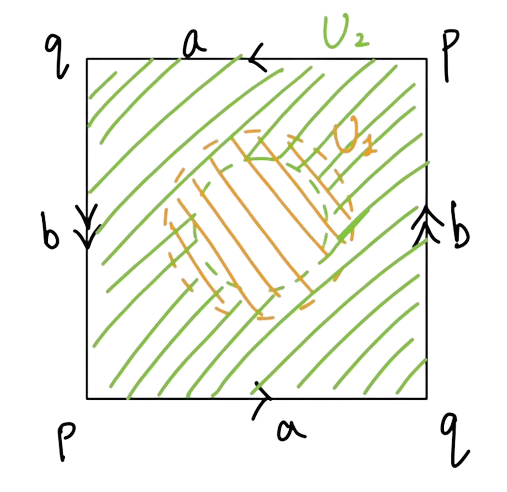
\includegraphics[scale = 0.3]{Image 1}
\end{center}

Notice that the green part $U_2$ which is a Mobius band deformation retracts to a circle with paths $a\cdot b\cdot a\cdot b$ while the orange disc $U_1$ is contractible. They have intersection $U_1\cap U_2$ that deformation retracts to $S^1$. Choose base point $x_0\in U_1\cap U_2$. Using Seifert-van Kampen's theorem, we have that $$\pi_1(\R\Prj^2,x_0)\cong1\ast_{\pi_1(U_1\cap U_2,x_0)}\Z$$ It remains to see how the amalgamated product is defined. Let $[\omega]$ be a generator of $\pi_1(U_1\cap U_2,x_0)$. Then $\omega$ is a simple loop in $U_1\cap U_2$. Notice the in $U_1$, $\omega$ deformation retracts to the constant loop and in $U_2$, $\omega$ deformation retracts to $a\cdot b\cdot a\cdot b$ the boundary. This means that $a\cdot b\cdot a\cdot b$ is identified as the identity by definition of the amalgamated product. Since $a\cdot b$ is a generator of $\pi_1(U_2,x_0)$, we have that $$\pi_1(\R\Prj^2,x_0)\cong\frac{\langle a\cdot b\rangle}{\langle a\cdot b\cdot a\cdot b\rangle}\cong\Z/2\Z$$ and so we conclude. 
\end{proof}
\end{thm}

A similar method can be employed for the torus and the Klein bottle. 














\end{document}
